\subsection{Dissecting the Differential IFIT2 Antibody Staining} \label{subsec:Dissecting the Differential IFIT2 Antibody Staining}
In Chapter \ref{ch:Subcellular Localisation of Endogenous IFIT Proteins in the Context of RSV Inclusion Bodies}, a striking differential staining pattern was observed between the two utilised anti-IFIT2 antibodies concerning the interaction of IFIT2 with human or bovine RSV inclusion bodies. The IFIT2(A) antibody revealed both human and bovine IFIT2 forming intra-IB inclusions in smaller IBs. Moreover, it observed IFIT2 to colocalise with the IB edge while being excluded from the IB centre in larger IBs. In contrast, IFIT2(B) predominantly detected IFIT2 to be excluded from IB structures, irrespective of IB size, occasionally showing IFIT2 to be equally distributed between the cytoplasm and IB structures. Additionally, a differential staining pattern was observed concerning the general subcellular localisation of IFIT2 in mock-treated cells, which was more pronounced in bovine cells. While both antibodies displayed general cytoplasmic staining of bovine IFIT2, IFIT2(A) staining revealed perinuclear concentrations resembling the Golgi apparatus. In contrast, IFIT2(B) antibody showed colocalisation of IFIT2 with the mitotic spindle. It appears that these two polyclonal antibodies are detecting two different entities, possibly two populations of IFIT2, basally present in both human and bovine cells. These populations may be detected by the antibodies based on differential epitope recognition. This difference could arise from one antibody detecting IFIT2 in complex with its interaction partners, such as IFIT1, IFIT3, MAVS, HOMER3, or double-stranded RNA, while the other antibody detects naked IFIT2 entities. The precise nature, however, remains to be elucidated.

To investigate this, we initially employed the same methodologies as were used in Section \ref{subsec:IFIT1, IFIT3, and IFIT5 Localisation with Regards to RSV Pseudo-IBs}. Specifically, we aimed to explore IFIT2 localisation concerning human and bovine RSV pseudo-inclusion bodies (pIBs), as detected by the IFIT2(A) and IFIT2(B) antibodies. We utilised the HEK293T and Vero cell lines to probe for endogenous human and monkey IFIT2, respectively. We induced hRSV pIBs in both HEK293T and Vero cell lines using the pcDNA3.1 plasmids containing ORFs for hRSV \textit{N} and \textit{P}. However, we encountered challenges in generating a sufficient amount of bRSV pIB-expressing Vero cells for staining with both IFIT2(A) and IFIT2(B) antibodies, and thus, the latter is missing from the analysis. This limitation may be attributed to contaminations in the plasmid preparations or a decrease in the quality of these plasmids.

\begin{figure}
    \centering
    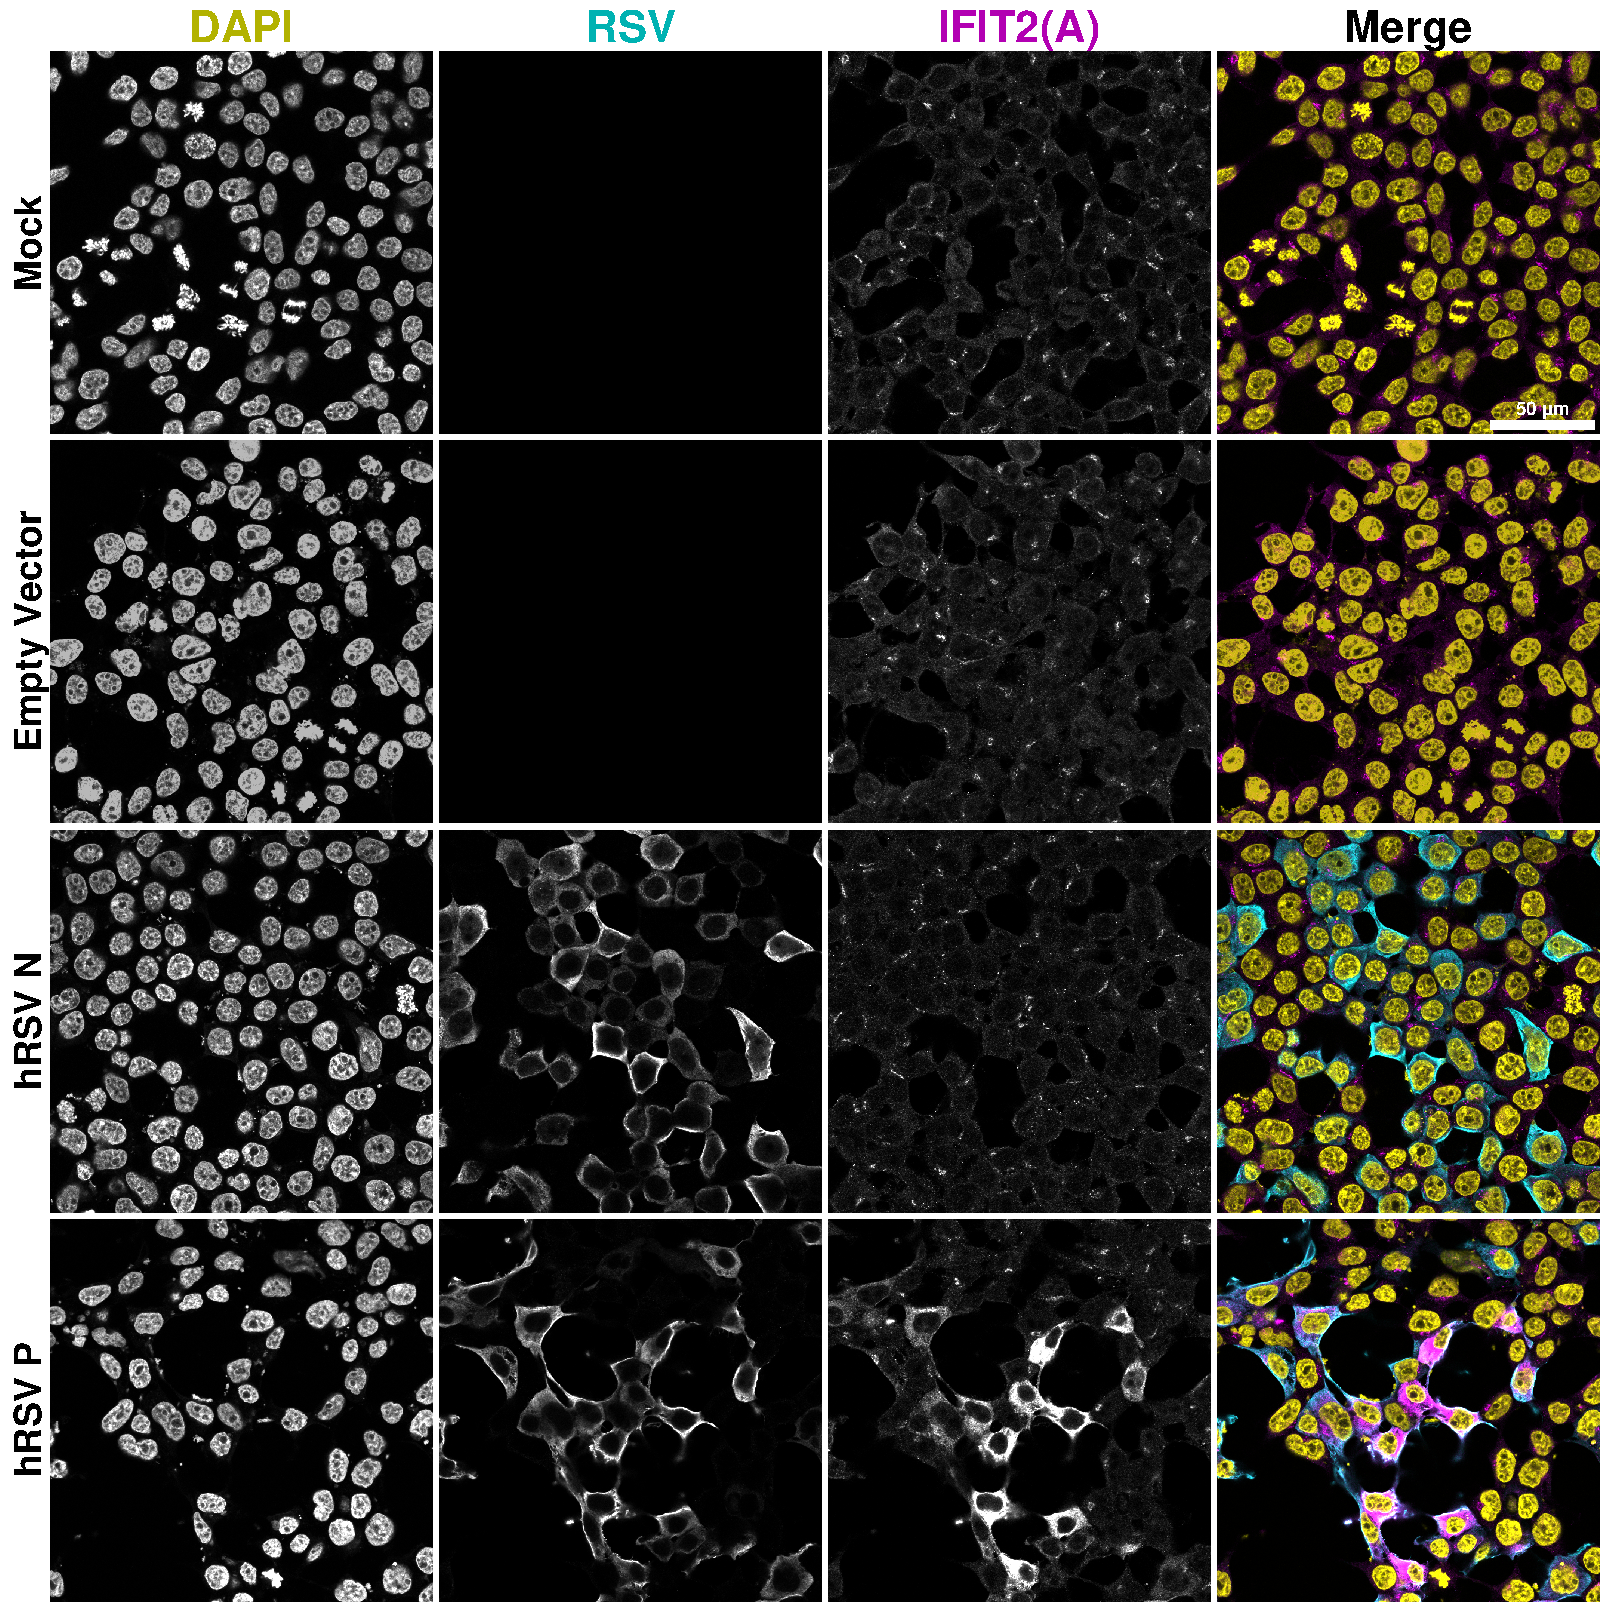
\includegraphics[width=1\linewidth]{09. Chapter 4/Figs/01. pIB/03. IFIT2/01. Single Transfection/01. 293t-ifit2a.pdf}
    \caption[IFIT2(A) Antibody Detects Increased IFIT2 Expression Following hRSV P Transfection.]{\textbf{IFIT2(A) Antibody Detects Increased IFIT2 Expression Following hRSV P Transfection.} HEK293T cells were either mock transfected, or single transfected with empty vector, hRSV N containing plasmid, or hRSV P containing plasmid using TransIT-X2 and were fixed after 24 hours. Cellular nuclei were stained with DAPI (yellow), and cells were double-labelled with either anti-RSV N (cyan), or anti-RSV P (cyan) and anti-IFIT2(A) (magenta) antibodies. The scale bar indicates 50 \(\mu \mbox{m}\).}
    \label{fig:IFIT2(A) Antibody Detects Increased IFIT2 Expression Following hRSV P Transfection}
\end{figure}

\begin{figure}
    \centering
    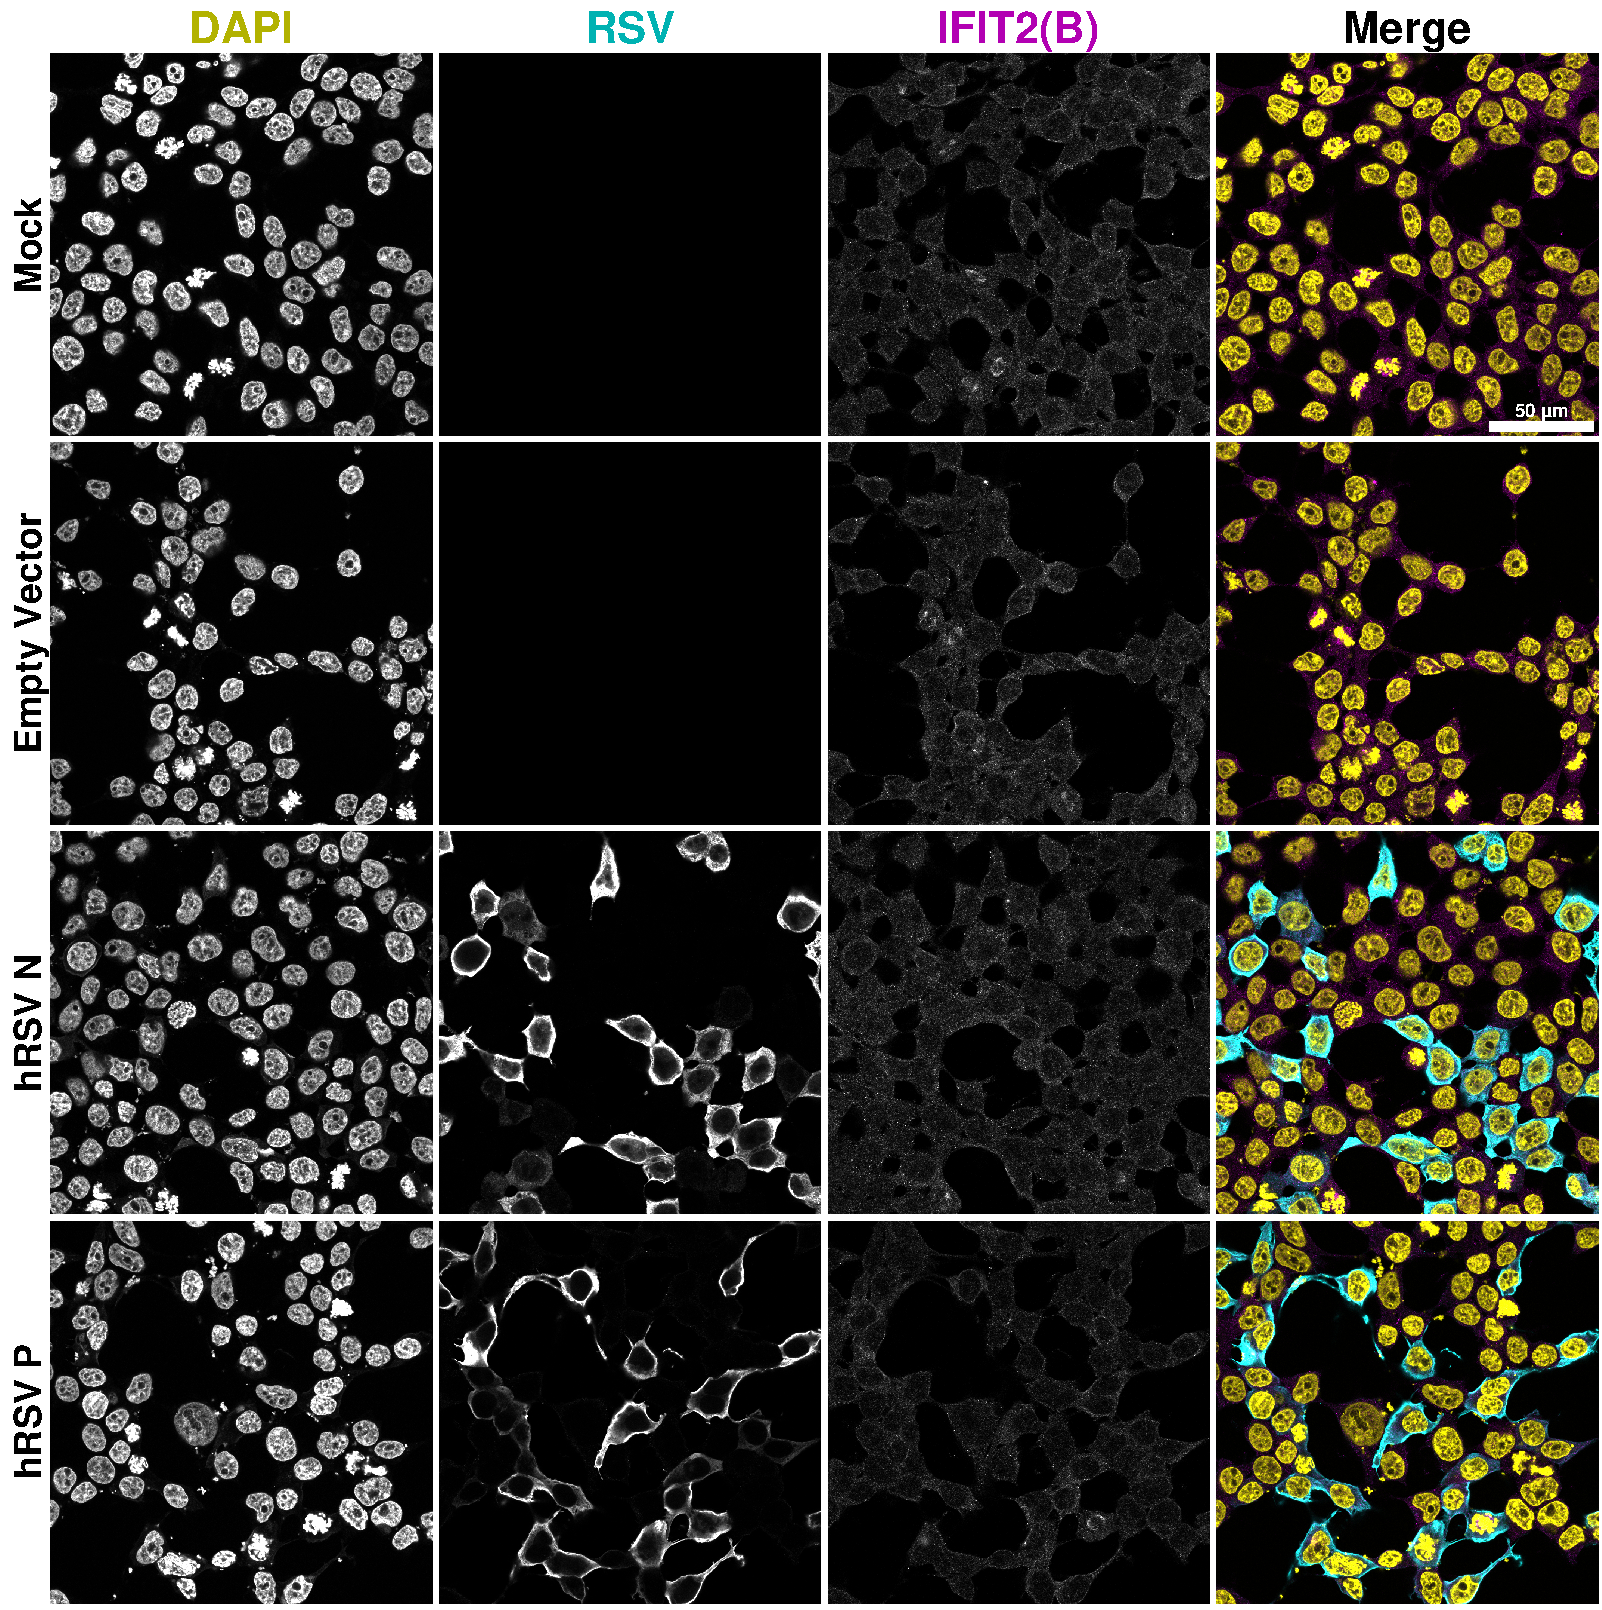
\includegraphics[width=1\linewidth]{09. Chapter 4/Figs/01. pIB/03. IFIT2/01. Single Transfection/02. 293t-ifit2b.pdf}
    \caption[IFIT2(B) Antibody Does Not Detect Increased IFIT2 Expression Following hRSV P Transfection.]{\textbf{IFIT2(B) Antibody Does Not Detect Increased IFIT2 Expression Following hRSV P Transfection.} HEK293T cells were either mock transfected, or single transfected with empty vector, hRSV N containing plasmid, or hRSV P containing plasmid using TransIT-X2 and were fixed after 24 hours. Cellular nuclei were stained with DAPI (yellow), and cells were double-labelled with either anti-RSV N (cyan), or anti-RSV P (cyan) and anti-IFIT2(B) (magenta) antibodies. The scale bar indicates 50 \(\mu \mbox{m}\).}
    \label{fig:IFIT2(B) Antibody Does Not Detect Increased IFIT2 Expression Following hRSV P Transfection}
\end{figure}

During the fundamental control experiments, which involved assessing single RSV \textit{N} and \textit{P} transfections and transfections with an empty pcDNA3.1 plasmid, while comparing these to mock-transfected cells, we uncovered a differentiation between IFIT2(A) and IFIT2(B) staining. Notably, we observed IFIT2 induction in response to transfection with the hRSV \textit{P}-containing plasmid, a response not observed during transfection with the empty vector or the hRSV \textit{N}-containing plasmid. This induction was detected exclusively using IFIT2(A) (Figure \ref{fig:IFIT2(A) Antibody Detects Increased IFIT2 Expression Following hRSV P Transfection}), while IFIT2(B) staining did not reveal this phenotype (Figure \ref{fig:IFIT2(B) Antibody Does Not Detect Increased IFIT2 Expression Following hRSV P Transfection}). Similar control experiments for IFIT1, IFIT3, and IFIT5 yielded staining patterns consistent with the observations made with IFIT2(B) antibody (data not shown). Additionally, we observed differential subcellular localisation of IFIT2 between the two antibodies, consistent with the findings in Chapter \ref{ch:Subcellular Localisation of Endogenous IFIT Proteins in the Context of RSV Inclusion Bodies} in the MDBK cell line. IFIT2(A)-stained HEK293T mock cells showed perinuclear IFIT2 concentrations resembling lipid droplets or aggregosomes, based on definitions and examples provided by the Human Protein Atlas \cite{Thul2017AProteome}. In contrast, IFIT2(B) antibody revealed IFIT2 localising to the mitotic spindle. This data raises several questions. Firstly, given that \textit{IFIT} genes should share similar genomic regulation, the mechanism through which \textit{IFIT2} is induced following RSV \textit{P} exogenous expression needs clarification. Is this induction mediated directly by the action of the P protein, suggesting its relevance to infection? Such a scenario would imply a potential direct antiviral role of IFIT2 against RSV. Secondly, the apparent inability of IFIT2(B) antibody to detect this increased nascent IFIT2 prompts further inquiry. If the previously mentioned differential target epitope hypothesis based on IFIT2 interaction partners holds true, it suggests that IFIT2(B) antibody detects IFIT2 complexes and is thus blind to newly synthesised IFIT2, which has not yet formed these complexes. Additional experiments are warranted to validate this proposition.

\begin{figure}
    \begin{subfigure}{0.495\textwidth}
        \caption{}
        \includegraphics[width=1\linewidth]{09. Chapter 4/Figs/01. pIB/03. IFIT2/02. IFIT2A/01. bar_i2a_293t.pdf}
    \end{subfigure}
    \begin{subfigure}{0.495\textwidth}
        \caption{}
        \includegraphics[width=1\linewidth]{09. Chapter 4/Figs/01. pIB/03. IFIT2/02. IFIT2A/02. box_i2a_293t.pdf}
    \end{subfigure}
    \caption[Observed Phenotypes of Endogenous Human IFIT2 in the Context of hRSV Pseudo Inclusion Bodies in 293T Cell Line, as Detected by IFIT2(A) Antibody.]{\textbf{Observed Phenotypes of Endogenous Human IFIT2 in the Context of hRSV Pseudo Inclusion Bodies in 293T Cell Line, as Detected by IFIT2(A) Antibody.} 293T cells were transfected with hRSV N and P containing plasmids using TransIT-X2 and were fixed after 24 hours. Cells were labelled with anti-RSV N and anti-IFIT2(A) antibodies and imaged on a confocal microscope. Panel (a) shows the percentual proportions of observed phenotypes between hRSV pseudo inclusion bodies and human IFIT2 (81 observations), with the red dotted line denoting the 5\% threshold, marking phenotypes considered relevant above this limit. Panel (b) shows the IB area in \(\mu \mbox{m}^2\) per observed relevant phenotype.}
    \label{fig:Observed Phenotypes of Endogenous Human IFIT2 in the Context of hRSV Pseudo Inclusion Bodies in 293T Cell Line, as Detected by IFIT2(A) Antibody}
\end{figure}

\begin{figure}
    \centering
    \includegraphics[width=1\linewidth]{09. Chapter 4/Figs/01. pIB/03. IFIT2/02. IFIT2A/03. i2a-293t-hnhp.pdf} 
    \caption[Representative Images of Observed Phenotypes of Endogenous Human IFIT2 in the Context of hRSV Pseudo Inclusion Bodies in 293T Cell Line, as Detected by IFIT2(A) Antibody.]{\textbf{Representative Images of Observed Phenotypes of Endogenous Human IFIT2 in the Context of hRSV Pseudo Inclusion Bodies in 293T Cell Line, as Detected by IFIT2(A) Antibody.} 293T cells were transfected with hRSV N and P containing plasmids using TransIT-X2 and were fixed after 24 hours. Cellular nuclei were stained with DAPI (yellow), and cells were double-labelled with anti-RSV N (cyan) and anti-IFIT2(A) (magenta) antibodies. This figure showcases representative examples of relevant phenotypes in the interaction between human IFIT2 and hRSV pseudo-inclusion bodies. These phenotypes are presented in descending order based on their percentage proportions. The scale bar indicates 2 \(\mu \mbox{m}\).}
    \label{fig:Representative Images of Observed Phenotypes of Endogenous Human IFIT2 in the Context of hRSV Pseudo Inclusion Bodies in 293T Cell Line, as Detected by IFIT2(A) Antibody}
\end{figure}

Next, we embarked on investigating the interaction phenotypes of IFIT2 with RSV pseudo IBs, as detected by the two antibodies. We initially focused on the signal identified by the IFIT2(A) antibody. We acquired 81 observations of human IFIT2 interacting with hRSV pIBs from the HEK293T cell line. Figure \ref{fig:Observed Phenotypes of Endogenous Human IFIT2 in the Context of hRSV Pseudo Inclusion Bodies in 293T Cell Line, as Detected by IFIT2(A) Antibody} displays the observed phenotypes, their frequencies of occurrences, and the pIB sizes associated with phenotypic interactions occurring with a frequency higher than 5\%. Representative images of phenotypes occurring at more than 5\% frequency are shown in Figure \ref{fig:Representative Images of Observed Phenotypes of Endogenous Human IFIT2 in the Context of hRSV Pseudo Inclusion Bodies in 293T Cell Line, as Detected by IFIT2(A) Antibody}. Predominantly, we observed IFIT2 forming intra-pIB inclusions, a phenotype occurring in 98\% of cases. In the remaining 2\% of observations, IFIT2 colocalised with the pIB boundary while being excluded from the pIB center. The sizes of inclusion-associated pIBs conformed to the general distribution of all observed pIBs in the HEK293T cell line, ranging from 0.1 \(\mu \mbox{m}^2\) to 25 \(\mu \mbox{m}^2\) in size, with a median area of 2 \(\mu \mbox{m}^2\). In contrast to observations with monkey IFIT1 and IFIT5, where the inclusion and colocalisation associated with exclusion phenotypes seemed to be restricted to small and large pIBs, respectively, we do not observe this distinction with endogenous human IFIT2. This suggests that IFIT2, as detected by the IFIT2(A) antibody, forms intra-pIB inclusions irrespective of their size.

\begin{figure}
    \begin{subfigure}{0.495\textwidth}
        \caption{}
        \includegraphics[width=1\linewidth]{09. Chapter 4/Figs/01. pIB/03. IFIT2/02. IFIT2A/04. bar_i2a_vero_hnhp.pdf} 
    \end{subfigure}
    \begin{subfigure}{0.495\textwidth}
        \caption{}
        \includegraphics[width=1\linewidth]{09. Chapter 4/Figs/01. pIB/03. IFIT2/02. IFIT2A/05. box_i2a_vero_hnhp.pdf}
    \end{subfigure}
    \caption[Observed Phenotypes of Endogenous Monkey IFIT2 in the Context of hRSV Pseudo Inclusion Bodies in Vero Cell Line, as Detected by IFIT2(A) Antibody.]{\textbf{Observed Phenotypes of Endogenous Monkey IFIT2 in the Context of hRSV Pseudo Inclusion Bodies in Vero Cell Line, as Detected by IFIT2(A) Antibody.} Vero cells were transfected with hRSV N and P containing plasmids using TransIT-X2 and were fixed after 24 hours. Cells were labelled with anti-RSV N and anti-IFIT2(A) antibodies and imaged on a confocal microscope. Panel (a) shows the percentual proportions of observed phenotypes between hRSV pseudo inclusion bodies and monkey IFIT2 (48 observations), with the red dotted line denoting the 5\% threshold, marking phenotypes considered relevant above this limit. Panel (b) shows the IB area in \(\mu \mbox{m}^2\) per observed relevant phenotype.}
    \label{fig:Observed Phenotypes of Endogenous Monkey IFIT2 in the Context of hRSV Pseudo Inclusion Bodies in Vero Cell Line, as Detected by IFIT2(A) Antibody}
\end{figure}

\begin{figure}
    \centering
    \includegraphics[width=1\linewidth]{09. Chapter 4/Figs/01. pIB/03. IFIT2/02. IFIT2A/06. i2a-vero-hnhp.pdf}  
    \caption[Representative Images of Observed Phenotypes of Endogenous Monkey IFIT2 in the Context of hRSV Pseudo Inclusion Bodies in Vero Cell Line, as Detected by IFIT2(A) Antibody.]{\textbf{Representative Images of Observed Phenotypes of Endogenous Monkey IFIT2 in the Context of hRSV Pseudo Inclusion Bodies in Vero Cell Line, as Detected by IFIT2(A) Antibody.} Vero cells were transfected with hRSV N and P containing plasmids using TransIT-X2 and were fixed after 24 hours. Cellular nuclei were stained with DAPI (yellow), and cells were double-labelled with anti-RSV N (cyan) and anti-IFIT2(A) (magenta) antibodies. This figure showcases representative examples of relevant phenotypes in the interaction between monkey IFIT2 and hRSV pseudo-inclusion bodies. These phenotypes are presented in descending order based on their percentage proportions. The scale bar indicates 2 \(\mu \mbox{m}\).}
    \label{fig:Representative Images of Observed Phenotypes of Endogenous Monkey IFIT2 in the Context of hRSV Pseudo Inclusion Bodies in Vero Cell Line, as Detected by IFIT2(A) Antibody}
\end{figure}

Further, we examined the interaction between monkey IFIT2 and hRSV pIBs using the IFIT2(A) antibody. To accomplish this, we transfected Vero cells with plasmids containing hRSV \textit{N} and \textit{P}. We obtained 48 observations, all of which conformed to the inclusion phenotype (Figure \ref{fig:Observed Phenotypes of Endogenous Monkey IFIT2 in the Context of hRSV Pseudo Inclusion Bodies in Vero Cell Line, as Detected by IFIT2(A) Antibody}, panel a). The measured area of these hRSV pIBs is shown in Figure \ref{fig:Observed Phenotypes of Endogenous Monkey IFIT2 in the Context of hRSV Pseudo Inclusion Bodies in Vero Cell Line, as Detected by IFIT2(A) Antibody}, panel b. The representative image is displayed in Figure \ref{fig:Representative Images of Observed Phenotypes of Endogenous Monkey IFIT2 in the Context of hRSV Pseudo Inclusion Bodies in Vero Cell Line, as Detected by IFIT2(A) Antibody}. The distribution of the pIB sizes is almost identical to the aggregate dataset of all pIBs observed in the Vero cell line, ranging from sub 0.07 \(\mu \mbox{m}^2\) to supra 60 \(\mu \mbox{m}^2\), with a typical value of 1.2 \(\mu \mbox{m}^2\). This data is consistent with our observations in HEK293T cells.

\begin{figure}
    \begin{subfigure}{0.495\textwidth}
        \caption{}
        \includegraphics[width=1\linewidth]{09. Chapter 4/Figs/01. pIB/03. IFIT2/02. IFIT2A/07. bar_i2a_vero_bnbp.pdf} 
    \end{subfigure}
    \begin{subfigure}{0.495\textwidth}
        \caption{}
        \includegraphics[width=1\linewidth]{09. Chapter 4/Figs/01. pIB/03. IFIT2/02. IFIT2A/08. box_i2a_vero_bnbp.pdf}
    \end{subfigure}
    \caption[Observed Phenotypes of Endogenous Monkey IFIT2 in the Context of bRSV Pseudo Inclusion Bodies in Vero Cell Line, as Detected by IFIT2(A) Antibody.]{\textbf{Observed Phenotypes of Endogenous Monkey IFIT2 in the Context of bRSV Pseudo Inclusion Bodies in Vero Cell Line, as Detected by IFIT2(A) Antibody.} Vero cells were transfected with bRSV N and P containing plasmids using TransIT-X2 and were fixed after 24 hours. Cells were labelled with anti-RSV N and anti-IFIT2(A) antibodies and imaged on a confocal microscope. Panel (a) shows the percentual proportions of observed phenotypes between bRSV pseudo inclusion bodies and monkey IFIT2 (38 observations), with the red dotted line denoting the 5\% threshold, marking phenotypes considered relevant above this limit. Panel (b) shows the IB area in \(\mu \mbox{m}^2\) per observed relevant phenotype.}
    \label{fig:Observed Phenotypes of Endogenous Monkey IFIT2 in the Context of bRSV Pseudo Inclusion Bodies in Vero Cell Line, as Detected by IFIT2(A) Antibody}
\end{figure}

\begin{figure}
    \centering
    \includegraphics[width=1\linewidth]{09. Chapter 4/Figs/01. pIB/03. IFIT2/02. IFIT2A/09. i2a-vero-bnbp.pdf} 
    \caption[Representative Images of Observed Phenotypes of Endogenous Monkey IFIT2 in the Context of bRSV Pseudo Inclusion Bodies in Vero Cell Line, as Detected by IFIT2(A) Antibody.]{\textbf{Representative Images of Observed Phenotypes of Endogenous Monkey IFIT2 in the Context of bRSV Pseudo Inclusion Bodies in Vero Cell Line, as Detected by IFIT2(A) Antibody.} Vero cells were transfected with bRSV N and P containing plasmids using TransIT-X2 and were fixed after 24 hours. Cellular nuclei were stained with DAPI (yellow), and cells were double-labelled with anti-RSV N (cyan) and anti-IFIT2(A) (magenta) antibodies. This figure showcases representative examples of relevant phenotypes in the interaction between monkey IFIT2 and bRSV pseudo-inclusion bodies. These phenotypes are presented in descending order based on their percentage proportions. The scale bar indicates 2 \(\mu \mbox{m}\).}
    \label{fig:Representative Images of Observed Phenotypes of Endogenous Monkey IFIT2 in the Context of bRSV Pseudo Inclusion Bodies in Vero Cell Line, as Detected by IFIT2(A) Antibody}
\end{figure}

Finally, we explored the interaction between monkey IFIT2 and bRSV pIBs using the IFIT2(A) antibody. This involved the transfection of Vero cells with bRSV \textit{N} and \textit{P} containing plasmids, resulting in 38 observations, all of which displayed the inclusion phenotype (Figure \ref{fig:Observed Phenotypes of Endogenous Monkey IFIT2 in the Context of bRSV Pseudo Inclusion Bodies in Vero Cell Line, as Detected by IFIT2(A) Antibody}, panel a). The measured area of these bRSV pIBs is illustrated in Figure \ref{fig:Observed Phenotypes of Endogenous Monkey IFIT2 in the Context of bRSV Pseudo Inclusion Bodies in Vero Cell Line, as Detected by IFIT2(A) Antibody}, panel b. Additionally, a representative image is provided in Figure \ref{fig:Representative Images of Observed Phenotypes of Endogenous Monkey IFIT2 in the Context of bRSV Pseudo Inclusion Bodies in Vero Cell Line, as Detected by IFIT2(A) Antibody}. While the observed pIBs may not perfectly represent the entirety of pIB observations in the Vero cell line, they span a significant range of pIB sizes. Consequently, we can confidently conclude that monkey IFIT2 forms intra-pIB inclusions regardless of the pIB's size. Specifically, these observed pIBs vary in size from 0.12 \(\mu \mbox{m}^2\) to 16 \(\mu \mbox{m}^2\), with a median value of 1.8 \(\mu \mbox{m}^2\). In summary, the IFIT2(A) antibody consistently detects IFIT2 forming intra-pIB inclusions, demonstrating the robustness of this interaction across different host cells, viral species, and pIB sizes.

\begin{figure}
    \begin{subfigure}{0.495\textwidth}
        \caption{}
        \includegraphics[width=1\linewidth]{09. Chapter 4/Figs/01. pIB/03. IFIT2/03. IFIT2B/01. bar_i2b_293t.pdf} 
    \end{subfigure}
    \begin{subfigure}{0.495\textwidth}
        \caption{}
        \includegraphics[width=1\linewidth]{09. Chapter 4/Figs/01. pIB/03. IFIT2/03. IFIT2B/02. box_i2b_293t.pdf}
    \end{subfigure}
    \caption[Observed Phenotypes of Endogenous Human IFIT2 in the Context of hRSV Pseudo Inclusion Bodies in 293T Cell Line, as Detected by IFIT2(B) Antibody.]{\textbf{Observed Phenotypes of Endogenous Human IFIT2 in the Context of hRSV Pseudo Inclusion Bodies in 293T Cell Line, as Detected by IFIT2(B) Antibody.} 293T cells were transfected with hRSV N and P containing plasmids using TransIT-X2 and were fixed after 24 hours. Cells were labelled with anti-RSV N and anti-IFIT2(B) antibodies and imaged on a confocal microscope. Panel (a) shows the percentual proportions of observed phenotypes between hRSV pseudo inclusion bodies and human IFIT2 (6 observations), with the red dotted line denoting the 5\% threshold, marking phenotypes considered relevant above this limit. Panel (b) shows the IB area in \(\mu \mbox{m}^2\) per observed relevant phenotype.}
    \label{fig:Observed Phenotypes of Endogenous Human IFIT2 in the Context of hRSV Pseudo Inclusion Bodies in 293T Cell Line, as Detected by IFIT2(B) Antibody}
\end{figure}

\begin{figure}
    \centering
    \includegraphics[width=1\linewidth]{09. Chapter 4/Figs/01. pIB/03. IFIT2/03. IFIT2B/03. i2b-293t-hnhp.pdf} 
    \caption[Representative Images of Observed Phenotypes of Endogenous Human IFIT2 in the Context of hRSV Pseudo Inclusion Bodies in 293T Cell Line, as Detected by IFIT2(B) Antibody.]{\textbf{Representative Images of Observed Phenotypes of Endogenous Human IFIT2 in the Context of hRSV Pseudo Inclusion Bodies in 293T Cell Line, as Detected by IFIT2(B) Antibody.} 293T cells were transfected with hRSV N and P containing plasmids using TransIT-X2 and were fixed after 24 hours. Cellular nuclei were stained with DAPI (yellow), and cells were double-labelled with anti-RSV N (cyan) and anti-IFIT2(B) (magenta) antibodies. This figure showcases representative examples of relevant phenotypes in the interaction between human IFIT2 and hRSV pseudo-inclusion bodies. These phenotypes are presented in descending order based on their percentage proportions. The scale bar indicates 2 \(\mu \mbox{m}\).}
    \label{fig:Representative Images of Observed Phenotypes of Endogenous Human IFIT2 in the Context of hRSV Pseudo Inclusion Bodies in 293T Cell Line, as Detected by IFIT2(B) Antibody}
\end{figure}

Next, we directed our attention to assessing the interaction of IFIT2 with hRSV pIBs, as detected by the IFIT2(B) antibody. Initially, we investigated the interaction of human IFIT2 with hRSV pIBs obtained from the HEK293T cell line. However, we obtained only 6 observations, all of which exhibited an exclusion phenotype (Figure \ref{fig:Observed Phenotypes of Endogenous Human IFIT2 in the Context of hRSV Pseudo Inclusion Bodies in 293T Cell Line, as Detected by IFIT2(B) Antibody}, panel a). The measured area of these hRSV pIBs is displayed in Figure \ref{fig:Observed Phenotypes of Endogenous Human IFIT2 in the Context of hRSV Pseudo Inclusion Bodies in 293T Cell Line, as Detected by IFIT2(B) Antibody}, panel b. The representative image of this phenotype is presented in Figure \ref{fig:Representative Images of Observed Phenotypes of Endogenous Human IFIT2 in the Context of hRSV Pseudo Inclusion Bodies in 293T Cell Line, as Detected by IFIT2(B) Antibody}. Although the observed pIBs were limited to 6, they encompass the range where the majority of the total observed hRSV pIB sizes were situated, ranging from sub 2 \(\mu \mbox{m}^2\) to supra 10 \(\mu \mbox{m}^2\), with a typical value of 4 \(\mu \mbox{m}^2\).

\begin{figure}
    \begin{subfigure}{0.495\textwidth}
        \caption{}
        \includegraphics[width=1\linewidth]{09. Chapter 4/Figs/01. pIB/03. IFIT2/03. IFIT2B/04. bar_i2b_vero_hnhp.pdf} 
    \end{subfigure}
    \begin{subfigure}{0.495\textwidth}
        \caption{}
        \includegraphics[width=1\linewidth]{09. Chapter 4/Figs/01. pIB/03. IFIT2/03. IFIT2B/05. box_i2b_vero_hnhp.pdf}
    \end{subfigure}
    \caption[Observed Phenotypes of Endogenous Monkey IFIT2 in the Context of hRSV Pseudo Inclusion Bodies in Vero Cell Line, as Detected by IFIT2(B) Antibody.]{\textbf{Observed Phenotypes of Endogenous Monkey IFIT2 in the Context of hRSV Pseudo Inclusion Bodies in Vero Cell Line, as Detected by IFIT2(B) Antibody.} Vero cells were transfected with hRSV N and P containing plasmids using TransIT-X2 and were fixed after 24 hours. Cells were labelled with anti-RSV N and anti-IFIT2(B) antibodies and imaged on a confocal microscope. Panel (a) shows the percentual proportions of observed phenotypes between hRSV pseudo inclusion bodies and monkey IFIT2 (76 observations), with the red dotted line denoting the 5\% threshold, marking phenotypes considered relevant above this limit. Panel (b) shows the IB area in \(\mu \mbox{m}^2\) per observed relevant phenotype.}
    \label{fig:Observed Phenotypes of Endogenous Monkey IFIT2 in the Context of hRSV Pseudo Inclusion Bodies in Vero Cell Line, as Detected by IFIT2(B) Antibody}
\end{figure}

\begin{figure}
    \centering
    \includegraphics[width=1\linewidth]{09. Chapter 4/Figs/01. pIB/03. IFIT2/03. IFIT2B/06. i2b-vero-hnhp.pdf} 
    \caption[Representative Images of Observed Phenotypes of Endogenous Monkey IFIT2 in the Context of hRSV Pseudo Inclusion Bodies in Vero Cell Line, as Detected by IFIT2(B) Antibody.]{\textbf{Representative Images of Observed Phenotypes of Endogenous Monkey IFIT2 in the Context of hRSV Pseudo Inclusion Bodies in Vero Cell Line, as Detected by IFIT2(B) Antibody.} Vero cells were transfected with hRSV N and P containing plasmids using TransIT-X2 and were fixed after 24 hours. Cellular nuclei were stained with DAPI (yellow), and cells were double-labelled with anti-RSV N (cyan) and anti-IFIT2(B) (magenta) antibodies. This figure showcases representative examples of relevant phenotypes in the interaction between monkey IFIT2 and hRSV pseudo-inclusion bodies. These phenotypes are presented in descending order based on their percentage proportions. The scale bar indicates 2 \(\mu \mbox{m}\).}
    \label{fig:Representative Images of Observed Phenotypes of Endogenous Monkey IFIT2 in the Context of hRSV Pseudo Inclusion Bodies in Vero Cell Line, as Detected by IFIT2(B) Antibody}
\end{figure}

Finally, we examined the interaction of endogenous monkey IFIT2 with hRSV pIBs, as detected by the IFIT2(B) antibody. Figure \ref{fig:Observed Phenotypes of Endogenous Monkey IFIT2 in the Context of hRSV Pseudo Inclusion Bodies in Vero Cell Line, as Detected by IFIT2(B) Antibody} presents the observed interaction phenotypes, their respective frequencies of occurrence, and the associated pIB sizes denoted per observed phenotype. Representative images of these interactions are shown in Figure \ref{fig:Representative Images of Observed Phenotypes of Endogenous Monkey IFIT2 in the Context of hRSV Pseudo Inclusion Bodies in Vero Cell Line, as Detected by IFIT2(B) Antibody}. Among the 76 observations, two phenotypes were identified: exclusion and diffusion. The former was predominant, appearing in 91\% of observations, while the latter occurred in 9\% of cases. The exclusion phenotype spanned a wide range of pIB sizes, representative of the aggregate distribution of all pIB sizes detected in the Vero cell line. Specifically, they ranged from 0.2 \(\mu \mbox{m}^2\) to 21 \(\mu \mbox{m}^2\), with a typical size of 2 \(\mu \mbox{m}^2\). The diffusion phenotype, however, predominantly occurred in smaller pIBs, ranging from 0.43 \(\mu \mbox{m}^2\) to 1 \(\mu \mbox{m}^2\), with a median size of 0.63 \(\mu \mbox{m}^2\).

Overall, our observations of IFIT2 interaction with RSV pIBs were consistent with those observed with endogenous human and bovine IFIT2 during RSV infection in Section \ref{subsec:Endogenous IFIT Interaction with RSV Inclusion Bodies}. The IFIT2(B) antibody detected endogenous human and monkey IFIT2 to be excluded from hRSV pIBs, with the exception of monkey IFIT2, where diffusion was also observed in 9\% of cases. In contrast, the IFIT2(A) antibody detected IFIT2 forming intra-pIBs solely, regardless of the host species or the species of the virus from which the pIBs originated. This differs from our observations during infection, where both human and bovine IFIT2, as detected by the IFIT2(A) antibody, were observed to form intra-IB inclusions in smaller IBs and to colocalise with the IB edge while being excluded from the IB interior in larger IBs. Nevertheless, a distinct difference is evident in observed IFIT2 using the two antibodies, and further investigation is needed to understand the nature of the differences observed by these antibodies. Employing a distinct epitope, such as the FLAG tag, could enhance our confidence in detecting the entire IFIT2 population.

To address this, we utilised the human IFIT2-FLAG-containing plasmid, provided by the Viral Gene Expression group at the Pirbright Institute, and the bovine IFIT2-FLAG-containing plasmid, prepared as described in Section \ref{sec:DNA Work} and Section \ref{subsec:Overexpressed IFIT1, IFIT3, and IFIT5 During RSV Infection}. We chose to initially assess these in the context of human and bovine RSV pseudo-inclusion bodies, as these yielded more defined interaction phenotypes as detected by the IFIT2(A) and IFIT2(B) antibodies. This approach also offers higher transfection efficiency compared to co-infection/transfection. After overexpressing the FLAG-tagged IFIT2, we aimed not only to probe the FLAG tag to obtain ground truth about IFIT2 subcellular localisation with respect to RSV pIBs but also to probe with the IFIT2(A) and IFIT2(B) antibodies to determine if their differential IFIT2 detection remains unchanged.

\begin{figure}
    \begin{subfigure}{0.495\textwidth}
        \caption{}
        \includegraphics[width=1\linewidth]{09. Chapter 4/Figs/01. pIB/03. IFIT2/04. IFIT2-FLAG/01. IFIT2A/01. bar_i2a_hnhp.pdf} 
    \end{subfigure}
    \begin{subfigure}{0.495\textwidth}
        \caption{}
        \includegraphics[width=1\linewidth]{09. Chapter 4/Figs/01. pIB/03. IFIT2/04. IFIT2-FLAG/01. IFIT2A/02. box_i2a_hnhp.pdf}
    \end{subfigure}
    \caption[Observed Phenotypes of Exogenous Human IFIT2 in the Context of hRSV Pseudo Inclusion Bodies in Vero Cell Line, as Detected by IFIT2(A) Antibody.]{\textbf{Observed Phenotypes of Exogenous Human IFIT2 in the Context of hRSV Pseudo Inclusion Bodies in Vero Cell Line, as Detected by IFIT2(A) Antibody.} Vero cells were transfected with hRSV N and P, along with human IFIT2-FLAG containing plasmids using TransIT-X2 and were fixed after 24 hours. Cells were labelled with anti-RSV N and anti-IFIT2(A) antibodies and imaged on a confocal microscope. Panel (a) shows the percentual proportions of observed phenotypes between hRSV pseudo inclusion bodies and exogenous human IFIT2 (56 observations), with the red dotted line denoting the 5\% threshold, marking phenotypes considered relevant above this limit. Panel (b) shows the IB area in \(\mu \mbox{m}^2\) per observed relevant phenotype.}
    \label{fig:Observed Phenotypes of Exogenous Human IFIT2 in the Context of hRSV Pseudo Inclusion Bodies in Vero Cell Line, as Detected by IFIT2(A) Antibody}
\end{figure}

\begin{figure}
    \centering
    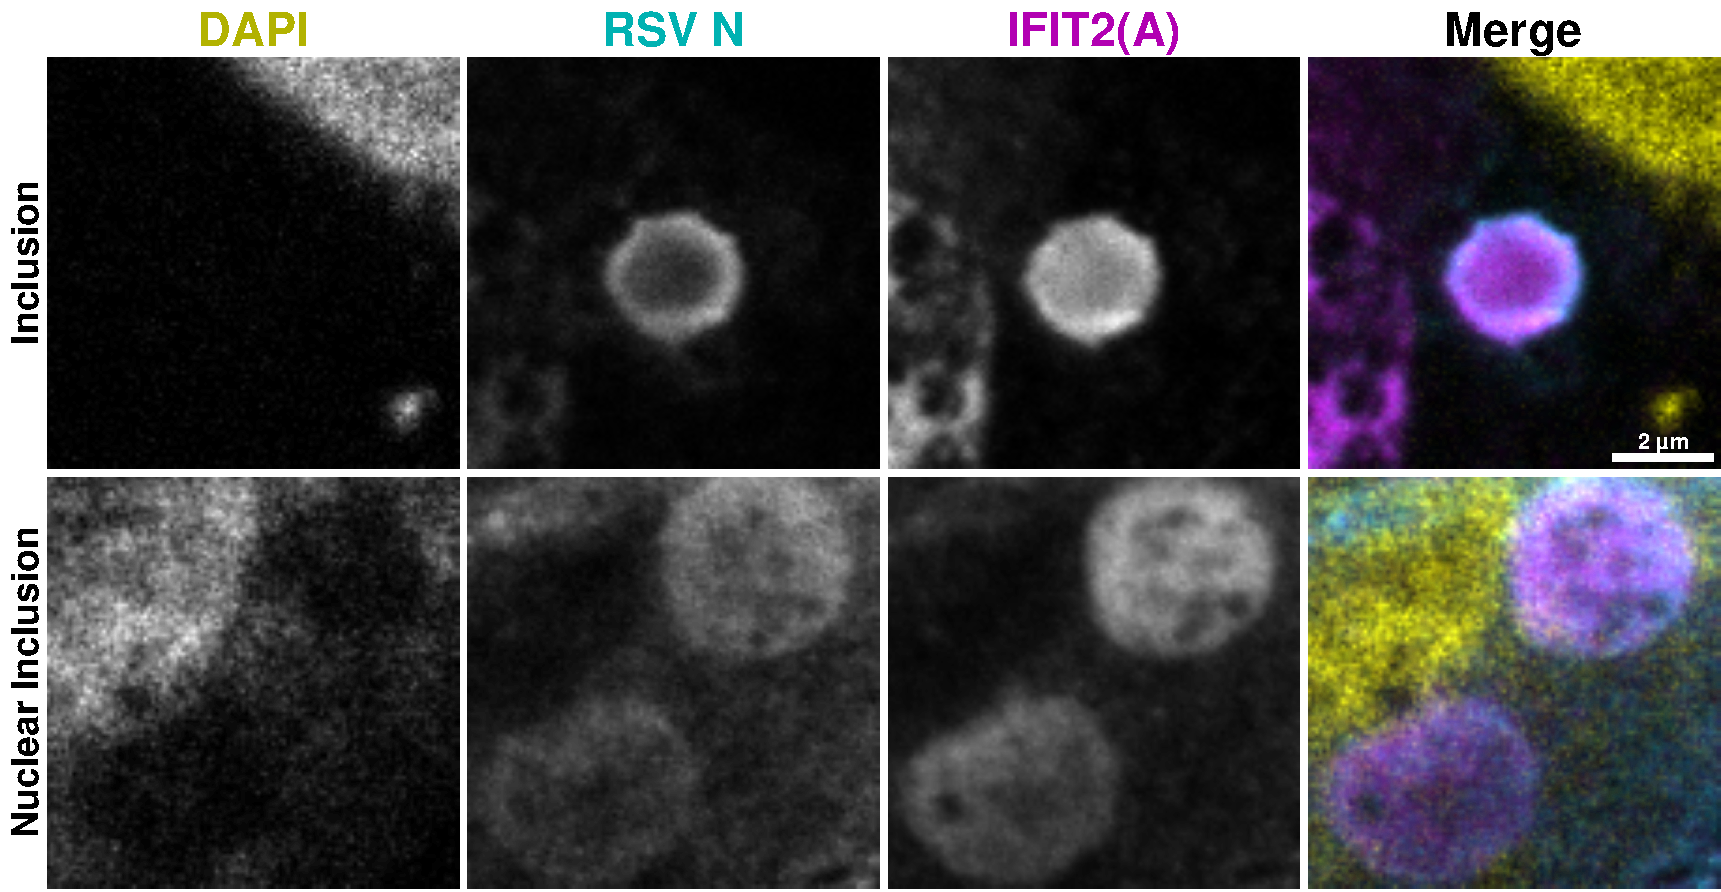
\includegraphics[width=1\linewidth]{09. Chapter 4/Figs/01. pIB/03. IFIT2/04. IFIT2-FLAG/01. IFIT2A/03. i2a-hi2f-hnhp.pdf}
    \caption[Representative Images of Observed Phenotypes of Exogenous Human IFIT2 in the Context of hRSV Pseudo Inclusion Bodies in Vero Cell Line, as Detected by IFIT2(A) Antibody.]{\textbf{Representative Images of Observed Phenotypes of Exogenous Human IFIT2 in the Context of hRSV Pseudo Inclusion Bodies in Vero Cell Line, as Detected by IFIT2(A) Antibody.} Vero cells were transfected with hRSV N and P, along with human IFIT2-FLAG containing plasmids using TransIT-X2 and were fixed after 24 hours. Cellular nuclei were stained with DAPI (yellow), and cells were double-labelled with anti-RSV N (cyan) and anti-IFIT2(A) (magenta) antibodies. This figure showcases representative examples of relevant phenotypes in the interaction between exogenous human IFIT2 and hRSV pseudo-inclusion bodies. These phenotypes are presented in descending order based on their percentage proportions. The scale bar indicates 2 \(\mu \mbox{m}\).}
    \label{fig:Representative Images of Observed Phenotypes of Exogenous Human IFIT2 in the Context of hRSV Pseudo Inclusion Bodies in Vero Cell Line, as Detected by IFIT2(A) Antibody}
\end{figure}

Initially, we expressed human IFIT2-FLAG in the context of hRSV pseudo-IBs in the Vero cell line and detected IFIT2 using the IFIT2(A) antibody. Successful transfection of hIFIT2-FLAG was determined by an increased IFIT2 signal compared to the surrounding cells (data not shown). We observed 56 instances, all displaying the inclusion phenotype (Figure \ref{fig:Observed Phenotypes of Exogenous Human IFIT2 in the Context of hRSV Pseudo Inclusion Bodies in Vero Cell Line, as Detected by IFIT2(A) Antibody}, panel a). The observed pIBs ranged in size from 0.09 \(\mu \mbox{m}^2\) to 29 \(\mu \mbox{m}^2\), with a median value of 0.9 \(\mu \mbox{m}^2\) (Figure \ref{fig:Observed Phenotypes of Exogenous Human IFIT2 in the Context of hRSV Pseudo Inclusion Bodies in Vero Cell Line, as Detected by IFIT2(A) Antibody}, panel b). Notably, we observed IFIT2 forming inclusions within nuclear pIBs as well, a phenomenon which will be described in more detail below. The representative images of cellular and nuclear inclusions are presented in Figure \ref{fig:Representative Images of Observed Phenotypes of Exogenous Human IFIT2 in the Context of hRSV Pseudo Inclusion Bodies in Vero Cell Line, as Detected by IFIT2(A) Antibody}.

\begin{figure}
    \begin{subfigure}{0.495\textwidth}
        \caption{}
        \includegraphics[width=1\linewidth]{09. Chapter 4/Figs/01. pIB/03. IFIT2/04. IFIT2-FLAG/02. IFIT2B/01. bar_i2b_hnhp.pdf}
    \end{subfigure}
    \begin{subfigure}{0.495\textwidth}
        \caption{}
        \includegraphics[width=1\linewidth]{09. Chapter 4/Figs/01. pIB/03. IFIT2/04. IFIT2-FLAG/02. IFIT2B/02. box_i2a_hnhp.pdf}
    \end{subfigure}
    \caption[Observed Phenotypes of Exogenous Human IFIT2 in the Context of hRSV Pseudo Inclusion Bodies in Vero Cell Line, as Detected by IFIT2(B) Antibody.]{\textbf{Observed Phenotypes of Exogenous Human IFIT2 in the Context of hRSV Pseudo Inclusion Bodies in Vero Cell Line, as Detected by IFIT2(B) Antibody.} Vero cells were transfected with hRSV N and P, along with human IFIT2-FLAG containing plasmids using TransIT-X2 and were fixed after 24 hours. Cells were labelled with anti-RSV N and anti-IFIT2(B) antibodies and imaged on a confocal microscope. Panel (a) shows the percentual proportions of observed phenotypes between hRSV pseudo inclusion bodies and exogenous human IFIT2 (44 observations), with the red dotted line denoting the 5\% threshold, marking phenotypes considered relevant above this limit. Panel (b) shows the IB area in \(\mu \mbox{m}^2\) per observed relevant phenotype.}
    \label{fig:Observed Phenotypes of Exogenous Human IFIT2 in the Context of hRSV Pseudo Inclusion Bodies in Vero Cell Line, as Detected by IFIT2(B) Antibody}
\end{figure}

\begin{figure}
    \centering
    \includegraphics[width=1\linewidth]{09. Chapter 4/Figs/01. pIB/03. IFIT2/04. IFIT2-FLAG/02. IFIT2B/03. i2b-hi2f-hnhp.pdf}
    \caption[Representative Images of Observed Phenotypes of Exogenous Human IFIT2 in the Context of hRSV Pseudo Inclusion Bodies in Vero Cell Line, as Detected by IFIT2(B) Antibody.]{\textbf{Representative Images of Observed Phenotypes of Exogenous Human IFIT2 in the Context of hRSV Pseudo Inclusion Bodies in Vero Cell Line, as Detected by IFIT2(B) Antibody.} Vero cells were transfected with hRSV N and P, along with human IFIT2-FLAG containing plasmids using TransIT-X2 and were fixed after 24 hours. Cellular nuclei were stained with DAPI (yellow), and cells were double-labelled with anti-RSV N (cyan) and anti-IFIT2(B) (magenta) antibodies. This figure showcases representative examples of relevant phenotypes in the interaction between exogenous human IFIT2 and hRSV pseudo-inclusion bodies. These phenotypes are presented in descending order based on their percentage proportions. The scale bar indicates 2 \(\mu \mbox{m}\).}
    \label{fig:Representative Images of Observed Phenotypes of Exogenous Human IFIT2 in the Context of hRSV Pseudo Inclusion Bodies in Vero Cell Line, as Detected by IFIT2(B) Antibody}
\end{figure}

Next, we replicated the previous experiment using the IFIT2(B) antibody for the detection of exogenous human IFIT2-FLAG. We obtained 44 observations of IFIT2-pIB interactions. The observed interactions, their frequencies of occurrence, along with the pIB sizes associated with phenotypes occurring with more than 5\% frequency, are illustrated in Figure \ref{fig:Observed Phenotypes of Exogenous Human IFIT2 in the Context of hRSV Pseudo Inclusion Bodies in Vero Cell Line, as Detected by IFIT2(B) Antibody}. Representative images of these interactions are shown in Figure \ref{fig:Representative Images of Observed Phenotypes of Exogenous Human IFIT2 in the Context of hRSV Pseudo Inclusion Bodies in Vero Cell Line, as Detected by IFIT2(B) Antibody}. Surprisingly, the most common interaction phenotype was inclusion, occurring in half of the observations. This was closely followed by the exclusion phenotype, which occurred in 47\% of cases. Lastly, we observed 3\% of observations conforming to the diffusion phenotype. While the inclusion phenotype occurred in pIBs of a broad size range, from 0.21 \(\mu \mbox{m}^2\) to 7.2 \(\mu \mbox{m}^2\), with a median value of 3.2 \(\mu \mbox{m}^2\), the exclusion phenotype occurred predominantly in smaller pIBs, ranging from sub 0.2 \(\mu \mbox{m}^2\) to 3.5 \(\mu \mbox{m}^2\), with a median value of 0.4 \(\mu \mbox{m}^2\). We observed the exclusion-associated pIBs to be located within the boundary of a nucleus. Taken together, both IFIT2(A) and IFIT2(B) antibodies detect exogenously expressed hIFIT2-FLAG forming intra-pIB inclusions. However, a discrepancy persists between the antibodies; IFIT2(A) detected IFIT2 forming inclusions within nuclear pIBs, while IFIT2(B) antibody observed IFIT2 to be excluded from these. Both antibodies did not detect IFIT2 within the nucleoplasm. Due to the persistent differential staining of the two antibodies, it is imperative to probe the exogenous IFIT2 using the anti-FLAG antibody.

\begin{figure}
    \begin{subfigure}{0.495\textwidth}
        \caption{}
        \includegraphics[width=1\linewidth]{09. Chapter 4/Figs/01. pIB/03. IFIT2/04. IFIT2-FLAG/03. FLAG/01. bar_hi2f_hnhp.pdf}
    \end{subfigure}
    \begin{subfigure}{0.495\textwidth}
        \caption{}
        \includegraphics[width=1\linewidth]{09. Chapter 4/Figs/01. pIB/03. IFIT2/04. IFIT2-FLAG/03. FLAG/02. box_hi2f_hnhp.pdf}
    \end{subfigure}
    \caption[Observed Phenotypes of Exogenous Human IFIT2 in the Context of hRSV Pseudo Inclusion Bodies in Vero Cell Line, as Detected by FLAG Antibody.]{\textbf{Observed Phenotypes of Exogenous Human IFIT2 in the Context of hRSV Pseudo Inclusion Bodies in Vero Cell Line, as Detected by FLAG Antibody.} Vero cells were transfected with hRSV N and P, along with human IFIT2-FLAG containing plasmids using TransIT-X2 and were fixed after 24 hours. Cells were labelled with anti-RSV N and anti-FLAG antibodies and imaged on a confocal microscope. Panel (a) shows the percentual proportions of observed phenotypes between hRSV pseudo inclusion bodies and exogenous human IFIT2 (116 observations), with the red dotted line denoting the 5\% threshold, marking phenotypes considered relevant above this limit. Panel (b) shows the IB area in \(\mu \mbox{m}^2\) per observed relevant phenotype.}
    \label{fig:Observed Phenotypes of Exogenous Human IFIT2 in the Context of hRSV Pseudo Inclusion Bodies in Vero Cell Line, as Detected by FLAG Antibody}
\end{figure}

\begin{figure}
    \centering
    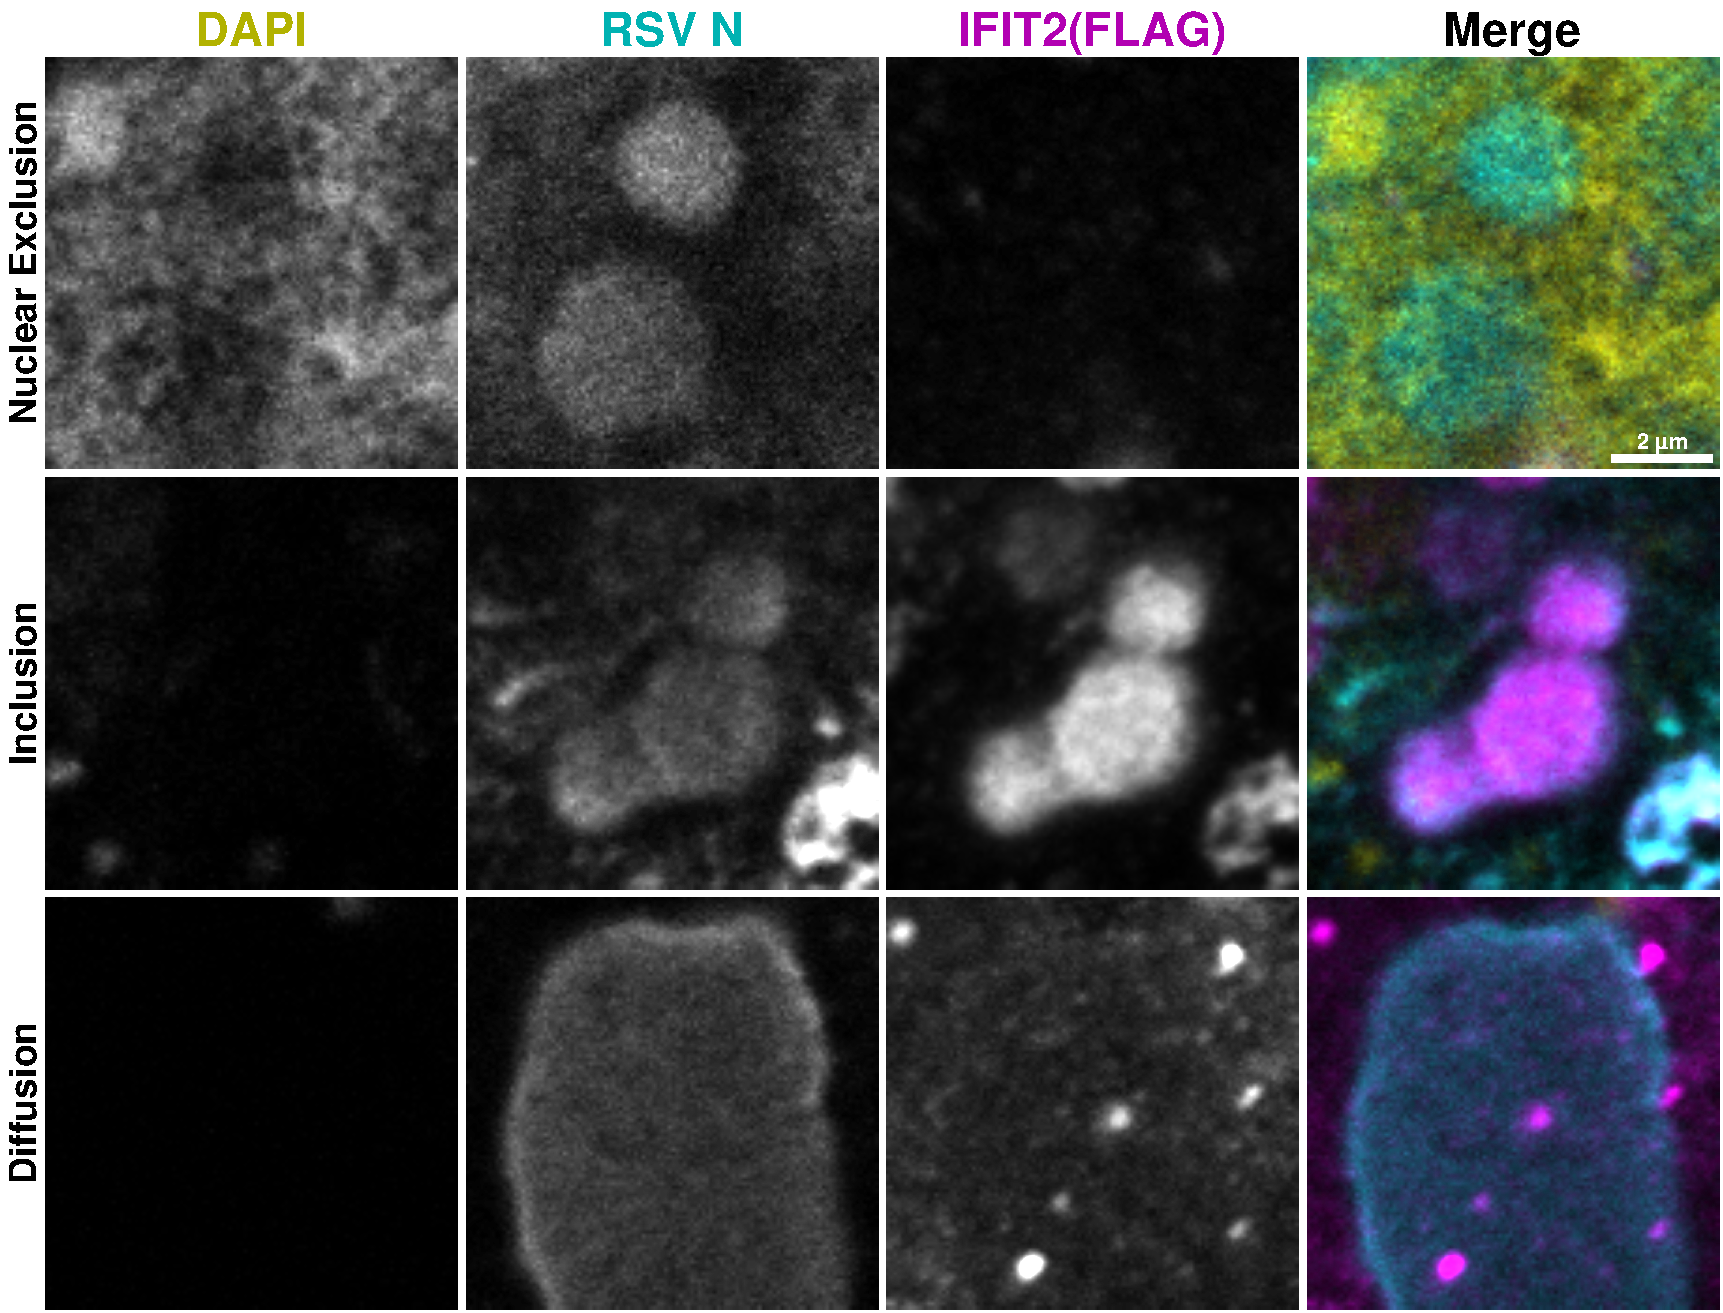
\includegraphics[width=1\linewidth]{09. Chapter 4/Figs/01. pIB/03. IFIT2/04. IFIT2-FLAG/03. FLAG/03. hi2f-hnhp.pdf}
    \caption[Representative Images of Observed Phenotypes of Exogenous Human IFIT2 in the Context of hRSV Pseudo Inclusion Bodies in Vero Cell Line, as Detected by FLAG Antibody.]{\textbf{Representative Images of Observed Phenotypes of Exogenous Human IFIT2 in the Context of hRSV Pseudo Inclusion Bodies in Vero Cell Line, as Detected by FLAG Antibody.} Vero cells were transfected with hRSV N and P, along with human IFIT2-FLAG containing plasmids using TransIT-X2 and were fixed after 24 hours. Cellular nuclei were stained with DAPI (yellow), and cells were double-labelled with anti-RSV N (cyan) and anti-FLAG (magenta) antibodies. This figure showcases representative examples of relevant phenotypes in the interaction between exogenous human IFIT2 and hRSV pseudo-inclusion bodies. These phenotypes are presented in descending order based on their percentage proportions. The scale bar indicates 2 \(\mu \mbox{m}\).}
    \label{fig:Representative Images of Observed Phenotypes of Exogenous Human IFIT2 in the Context of hRSV Pseudo Inclusion Bodies in Vero Cell Line, as Detected by FLAG Antibody}
\end{figure}

Using the anti-FLAG antibody, we probed the true localisation of exogenously expressed human IFIT2-FLAG and its interaction with hRSV pIBs. The frequencies of occurrences of observed interaction phenotypes, based on 116 observations, along with the measured pIB sizes associated with the phenotypes, are depicted in Figure \ref{fig:Observed Phenotypes of Exogenous Human IFIT2 in the Context of hRSV Pseudo Inclusion Bodies in Vero Cell Line, as Detected by FLAG Antibody}. Representative images of these phenotypes are shown in Figure \ref{fig:Representative Images of Observed Phenotypes of Exogenous Human IFIT2 in the Context of hRSV Pseudo Inclusion Bodies in Vero Cell Line, as Detected by FLAG Antibody}. The most common phenotype was exclusion from the pIB structures, occurring in 49\% of observations. This was followed by intra-pIB inclusions, occurring at a frequency of 35\%. Lastly, we detected IFIT2 to be diffused equally throughout the cytoplasm and the pIB structure in 21\% of observations. Exclusion appeared predominantly in smaller sub 1 \(\mu \mbox{m}^2\) pIBs, although we observed 4 pIBs associated with this phenotype that were larger than this. In more detail, exclusion-associated pIBs ranged from 0.09 \(\mu \mbox{m}^2\) to 9 \(\mu \mbox{m}^2\), with a typical value of 0.23 \(\mu \mbox{m}^2\). These pIBs were also located within the boundary of the nucleus. The inclusion-associated pIBs ranged from 0.2 \(\mu \mbox{m}^2\) to 9 \(\mu \mbox{m}^2\), with a median value of 2.1 \(\mu \mbox{m}^2\). Lastly, while the diffusion phenotype occurred predominantly with small, sub 1 \(\mu \mbox{m}^2\) pIBs, we observed 6 outliers that were each progressively larger. In general, the diffusion-associated pIBs ranged from 0.09 \(\mu \mbox{m}^2\) to 55 \(\mu \mbox{m}^2\), with a median value of just 0.7 \(\mu \mbox{m}^2\).

These data are consistent with what was observed in overexpressed hIFIT2-FLAG as detected by the IFIT2(B) antibody, suggesting that this antibody more realistically portrays the IFIT2 population. It is intriguing that ectopic expression of IFIT2 suddenly enables the IFIT2(B) antibody to detect IFIT2 forming intra-pIB inclusions. This observation is difficult to explain, but we suspect it may result from exogenous IFIT2-FLAG losing some of its interaction partners, potentially due to the C-terminal FLAG tag. This data also indicates that our previous assumption was correct, meaning the real interaction of IFIT2 with both IB and pIB involves both exclusion and strong interaction phenotypes (inclusion or colocalisation associated with exclusion), occurring approximately in the same frequency. Another intriguing fact is that while both IFIT2(B) and FLAG antibodies did not detect IFIT2 interaction with the nucleus-associated pIBs, the IFIT2(A) antibody was able to detect inclusions. This could possibly be explained by IFIT2(A) off-target effects or by some mechanism which we do not comprehend yet.

\begin{figure}
    \begin{subfigure}{0.495\textwidth}
        \caption{}
        \includegraphics[width=1\linewidth]{09. Chapter 4/Figs/01. pIB/03. IFIT2/04. IFIT2-FLAG/03. FLAG/04. bar_bi2f_hnhp.pdf} 
    \end{subfigure}
    \begin{subfigure}{0.495\textwidth}
        \caption{}
        \includegraphics[width=1\linewidth]{09. Chapter 4/Figs/01. pIB/03. IFIT2/04. IFIT2-FLAG/03. FLAG/05. box_bi2f_hnhp.pdf}
    \end{subfigure}
    \caption[Observed Phenotypes of Exogenous Bovine IFIT2 in the Context of hRSV Pseudo Inclusion Bodies in Vero Cell Line, as Detected by FLAG Antibody.]{\textbf{Observed Phenotypes of Exogenous Bovine IFIT2 in the Context of hRSV Pseudo Inclusion Bodies in Vero Cell Line, as Detected by FLAG Antibody.} Vero cells were transfected with hRSV N (or N-GFP) and P, along with bovine IFIT2-FLAG containing plasmids using TransIT-X2 and were fixed after 24 hours. Cells were labelled with anti-RSV N and anti-FLAG antibodies and imaged on a confocal microscope. The N-GFP containing pIBs were visualised using the innate fluorescence of the GFP. Panel (a) shows the percentual proportions of observed phenotypes between hRSV pseudo inclusion bodies and exogenous bovine IFIT2 (142 observations), with the red dotted line denoting the 5\% threshold, marking phenotypes considered relevant above this limit. Panel (b) shows the IB area in \(\mu \mbox{m}^2\) per observed relevant phenotype.}
    \label{fig:Observed Phenotypes of Exogenous Bovine IFIT2 in the Context of hRSV Pseudo Inclusion Bodies in Vero Cell Line, as Detected by FLAG Antibody}
\end{figure}

\begin{figure}
    \centering
    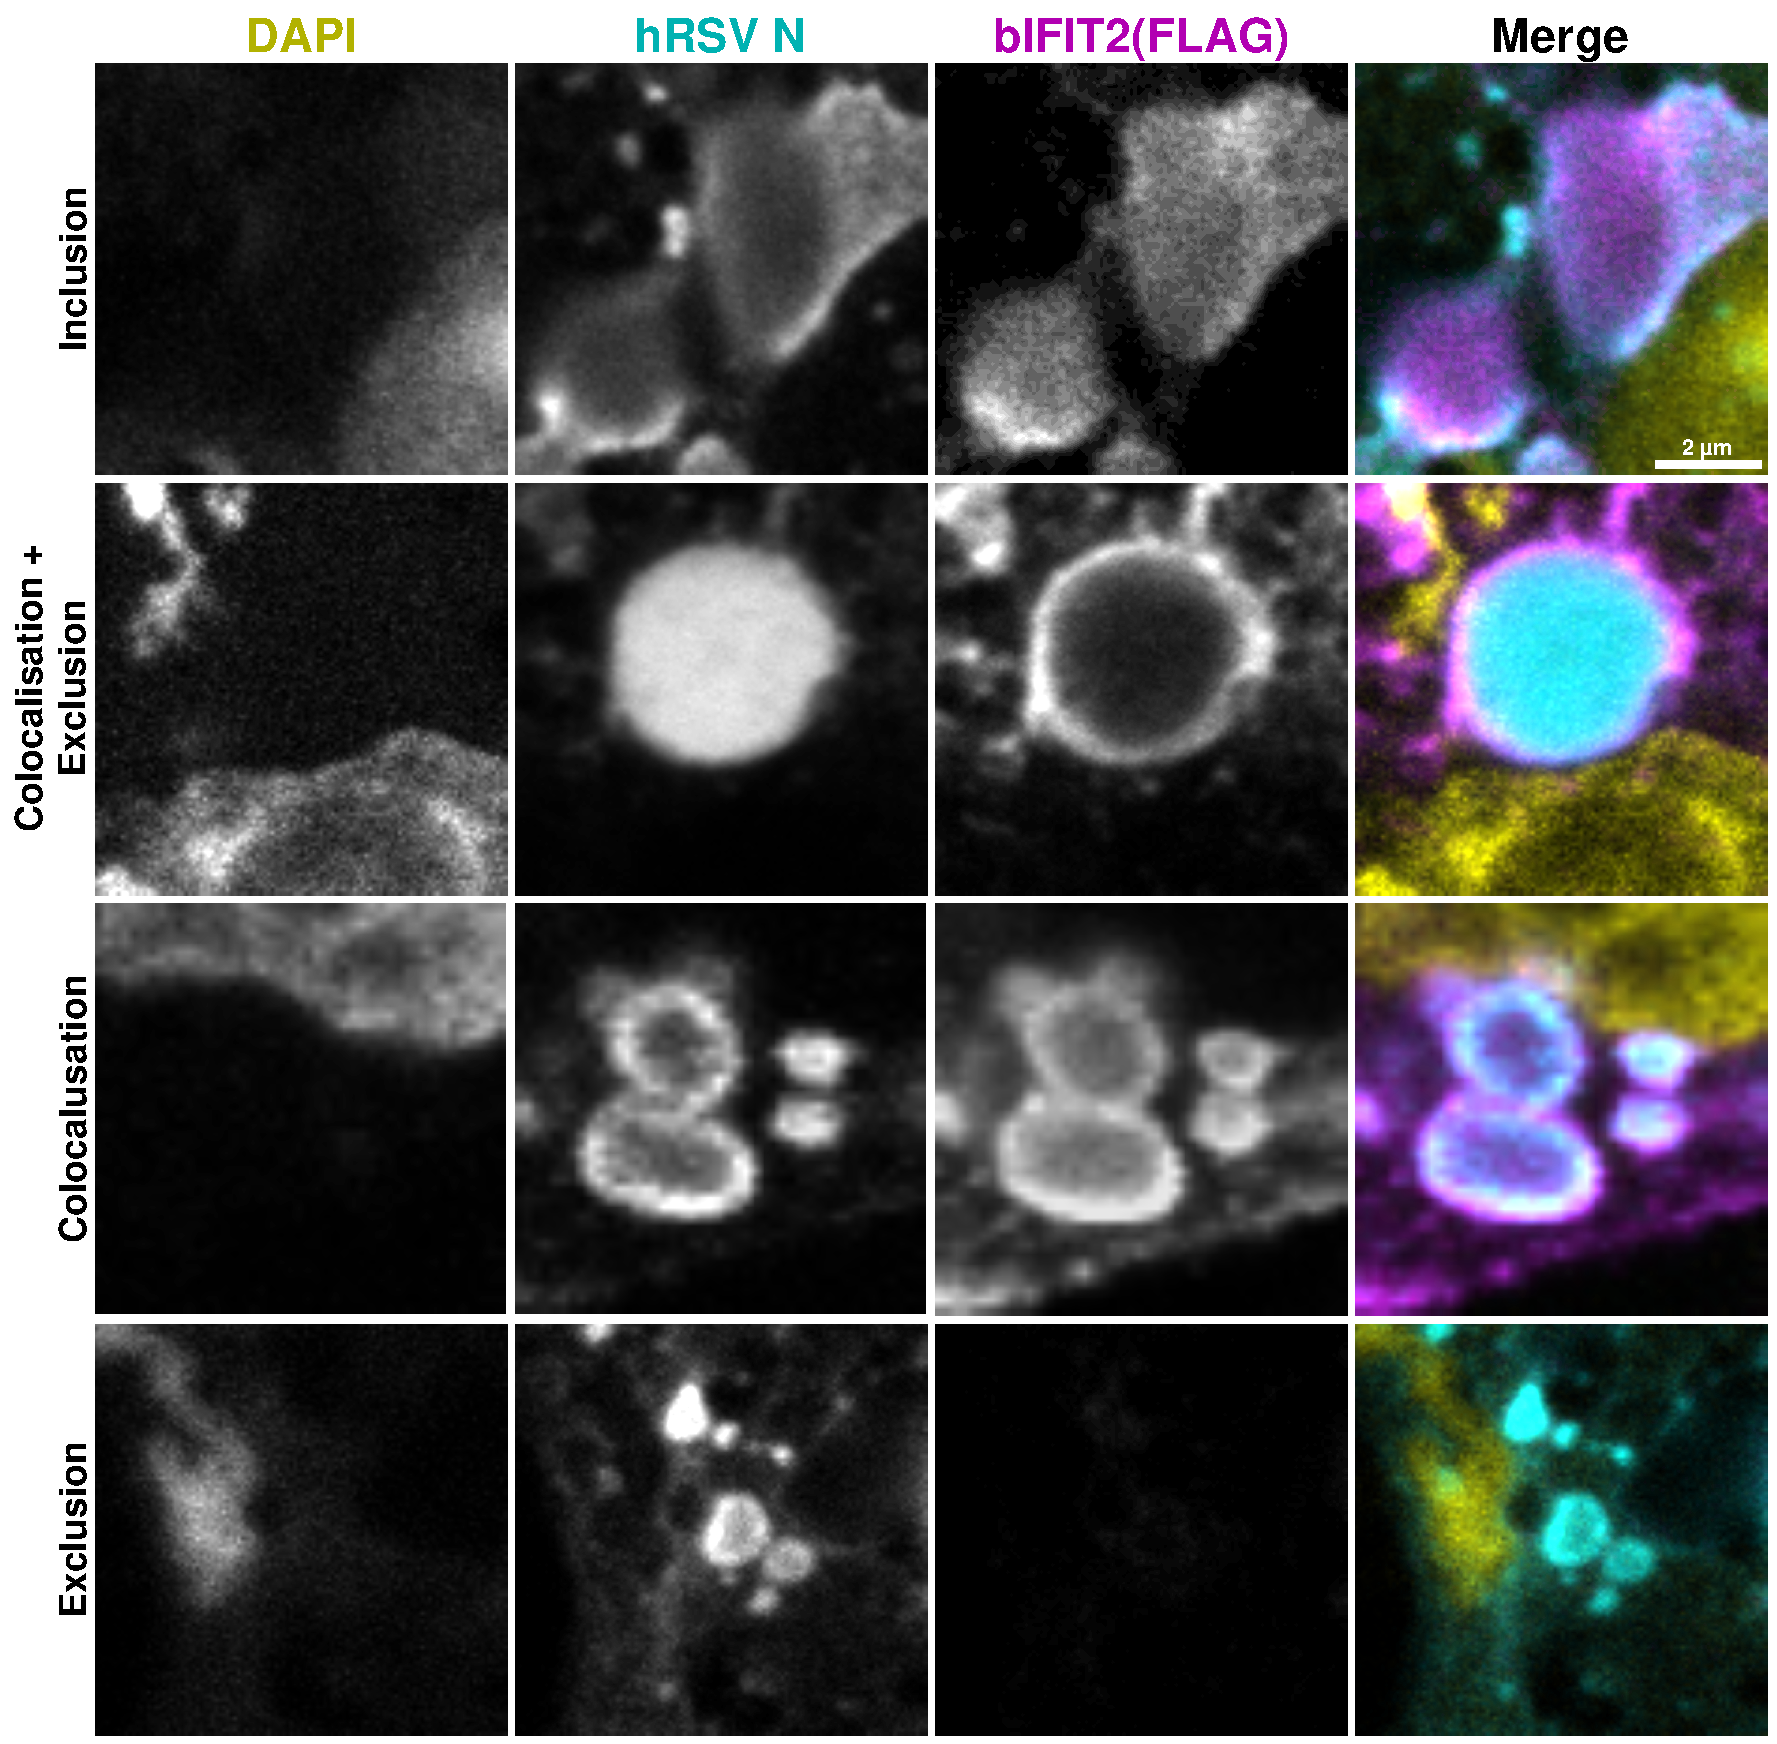
\includegraphics[width=1\linewidth]{09. Chapter 4/Figs/01. pIB/03. IFIT2/04. IFIT2-FLAG/03. FLAG/06. bi2f-hnhp.pdf}
    \caption[Representative Images of Observed Phenotypes of Exogenous Bovine IFIT2 in the Context of hRSV Pseudo Inclusion Bodies in Vero Cell Line, as Detected by FLAG Antibody.]{\textbf{Representative Images of Observed Phenotypes of Exogenous Bovine IFIT2 in the Context of hRSV Pseudo Inclusion Bodies in Vero Cell Line, as Detected by FLAG Antibody.} Vero cells were transfected with hRSV N (or N-GFP) and P, along with bovine IFIT2-FLAG containing plasmids using TransIT-X2 and were fixed after 24 hours. Cellular nuclei were stained with DAPI (yellow), and cells were double-labelled with anti-RSV N (cyan) and anti-FLAG (magenta) antibodies. The N-GFP containing pIBs were visualised using the innate fluorescence of the GFP (colocalisation + exclusion phenotype). This figure showcases representative examples of relevant phenotypes in the interaction between exogenous bovine IFIT2 and hRSV pseudo-inclusion bodies. These phenotypes are presented in descending order based on their percentage proportions. The scale bar indicates 2 \(\mu \mbox{m}\).}
    \label{fig:Representative Images of Observed Phenotypes of Exogenous Bovine IFIT2 in the Context of hRSV Pseudo Inclusion Bodies in Vero Cell Line, as Detected by FLAG Antibody}
\end{figure}

We continued the investigation of IFIT2-FLAG interaction with pIB structures, focusing solely on the FLAG antibody for detection. Attempts to obtain data from exogenous human IFIT2-FLAG with regards to bRSV pIBs were unsuccessful, as we failed to detect a single cell co-transfected by all three required plasmids. Consequently, we proceeded with the investigation involving exogenously expressed bovine IFIT2-FLAG in the context of human and bovine RSV pseudo-inclusion bodies. Firstly, we explored overexpressed bIFIT2-FLAG and its interaction with hRSV pIBs induced by co-transfecting RSV \textit{P}-containing plasmid with either hRSV \textit{N}- or \textit{N-GFP}-containing plasmids. The GFP signal, which is more sensitive, revealed N being distributed through the pIB. These samples, obtained from the Vero cell line, were detected using the anti-FLAG antibody. We obtained 142 observations of bIFIT2-hRSV pIB interactions, revealing a diverse range of interaction phenotypes. These phenotypes, along with their occurrence frequencies and the measured sizes of pIBs per observed phenotype occurring with more than 5\% frequency, are illustrated in Figure \ref{fig:Observed Phenotypes of Exogenous Bovine IFIT2 in the Context of hRSV Pseudo Inclusion Bodies in Vero Cell Line, as Detected by FLAG Antibody}. Representative images of these phenotypes are shown in Figure \ref{fig:Representative Images of Observed Phenotypes of Exogenous Bovine IFIT2 in the Context of hRSV Pseudo Inclusion Bodies in Vero Cell Line, as Detected by FLAG Antibody}.

We observed bovine IFIT2-FLAG to form intra-pIB inclusions in 46\% of all observations. This was followed by the colocalisation associated with exclusion phenotype, occurring in 31\% of cases, predominantly in pIBs created using the transfection of hRSV \textit{P} and \textit{N-GFP} containing plasmids. The next most prevalent phenotype was colocalisation, which occurred in 12\% of observations. Therefore, exogenous bovine IFIT2 displays strong interaction phenotypes with an 89\% frequency. The remaining 11\% of observations consisted of exclusion (6\%), edge exclusion (4\%), and diffusion (1\%) phenotypes. Inclusion occurred in pIBs spanning the entire size spectrum, from sub 0.2 \(\mu \mbox{m}^2\) to a maximum of 120 \(\mu \mbox{m}^2\), with a median value of 1 \(\mu \mbox{m}^2\). This phenotype was the most common among all pIBs smaller than 1 \(\mu \mbox{m}^2\) and was the only phenotype occurring in pIBs sub 0.5 \(\mu \mbox{m}^2\) in size. The colocalisation associated with exclusion phenotype occurred in pIBs ranging from 0.9 \(\mu \mbox{m}^2\) to 21 \(\mu \mbox{m}^2\) in size, with a typical value of 2.8 \(\mu \mbox{m}^2\). The same median value was observed for the colocalisation phenotype; however, the overall distribution shifted towards smaller sizes, ranging from 0.7 \(\mu \mbox{m}^2\) to 7.5 \(\mu \mbox{m}^2\). Lastly, the exclusion phenotype displayed the most compact size range, from 0.53 \(\mu \mbox{m}^2\) to sub 3 \(\mu \mbox{m}^2\), with a median value of 1.7 \(\mu \mbox{m}^2\). This data suggests a size separation of observed phenotypes, where IFIT2 associated with small pIBs forms inclusions inside them, while the IFIT2 associated with medium-sized pIBs mainly conforms to colocalisation phenotypes, either without or with associated exclusion.

\begin{figure}
    \begin{subfigure}{0.495\textwidth}
        \caption{}
        \includegraphics[width=1\linewidth]{09. Chapter 4/Figs/01. pIB/03. IFIT2/04. IFIT2-FLAG/03. FLAG/07. bar_bi2f_bnbp.pdf} 
    \end{subfigure}
    \begin{subfigure}{0.495\textwidth}
        \caption{}
        \includegraphics[width=1\linewidth]{09. Chapter 4/Figs/01. pIB/03. IFIT2/04. IFIT2-FLAG/03. FLAG/08. box_bi2f_bnbp.pdf}
    \end{subfigure}
    \caption[Observed Phenotypes of Exogenous Bovine IFIT2 in the Context of bRSV Pseudo Inclusion Bodies in Vero Cell Line, as Detected by FLAG Antibody.]{\textbf{Observed Phenotypes of Exogenous Bovine IFIT2 in the Context of bRSV Pseudo Inclusion Bodies in Vero Cell Line, as Detected by FLAG Antibody.} Vero cells were transfected with bRSV N and P, along with bovine IFIT2-FLAG containing plasmids using TransIT-X2 and were fixed after 24 hours. Cells were labelled with anti-RSV N and anti-FLAG antibodies and imaged on a confocal microscope. Panel (a) shows the percentual proportions of observed phenotypes between bRSV pseudo inclusion bodies and exogenous bovine IFIT2 (22 observations), with the red dotted line denoting the 5\% threshold, marking phenotypes considered relevant above this limit. Panel (b) shows the IB area in \(\mu \mbox{m}^2\) per observed relevant phenotype.}
    \label{fig:Observed Phenotypes of Exogenous Bovine IFIT2 in the Context of bRSV Pseudo Inclusion Bodies in Vero Cell Line, as Detected by FLAG Antibody}
\end{figure}

\begin{figure}
    \centering
    \includegraphics[width=1\linewidth]{09. Chapter 4/Figs/01. pIB/03. IFIT2/04. IFIT2-FLAG/03. FLAG/09. bi2f-bnbp.pdf}
    \caption[Representative Images of Observed Phenotypes of Exogenous Bovine IFIT2 in the Context of bRSV Pseudo Inclusion Bodies in Vero Cell Line, as Detected by FLAG Antibody.]{\textbf{Representative Images of Observed Phenotypes of Exogenous Bovine IFIT2 in the Context of bRSV Pseudo Inclusion Bodies in Vero Cell Line, as Detected by FLAG Antibody.} Vero cells were transfected with bRSV N and P, along with bovine IFIT2-FLAG containing plasmids using TransIT-X2 and were fixed after 24 hours. Cellular nuclei were stained with DAPI (yellow), and cells were double-labelled with anti-RSV N (cyan) and anti-FLAG (magenta) antibodies. This figure showcases representative examples of relevant phenotypes in the interaction between exogenous bovine IFIT2 and bRSV pseudo-inclusion bodies. These phenotypes are presented in descending order based on their percentage proportions. The scale bar indicates 2 \(\mu \mbox{m}\).}
    \label{fig:Representative Images of Observed Phenotypes of Exogenous Bovine IFIT2 in the Context of bRSV Pseudo Inclusion Bodies in Vero Cell Line, as Detected by FLAG Antibody}
\end{figure}

Finally, we explored the phenotypic interactions resulting from the exogenous expression of bovine IFIT2-FLAG in conjunction with bRSV pIBs, as detected by the anti-FLAG antibody. Due to challenges encountered during bRSV \textit{P} and \textit{N}-containing plasmid transfection, our dataset comprises only 22 observations. All of these observations consistently revealed IFIT2 forming intra-pIB inclusions (Figure \ref{fig:Observed Phenotypes of Exogenous Bovine IFIT2 in the Context of bRSV Pseudo Inclusion Bodies in Vero Cell Line, as Detected by FLAG Antibody}, panel a). The representative image of this interaction is displayed in Figure \ref{fig:Representative Images of Observed Phenotypes of Exogenous Bovine IFIT2 in the Context of bRSV Pseudo Inclusion Bodies in Vero Cell Line, as Detected by FLAG Antibody}. Intriguingly, predominantly small pIBs were observed in this dataset, ranging from 0.11 $\mu \mbox{m}^2$ to 3.5 $\mu \mbox{m}^2$, with a median size of only 0.41 $\mu \mbox{m}^2$ (Figure \ref{fig:Observed Phenotypes of Exogenous Bovine IFIT2 in the Context of bRSV Pseudo Inclusion Bodies in Vero Cell Line, as Detected by FLAG Antibody}, panel b). It is plausible that with the observation of larger pIBs, IFIT2 would interact by colocalising with their boundaries, similar to our observations with hRSV pIBs.

Collectively, we assert that probing for the localisation of exogenous human and bovine IFIT2-FLAG with the anti-FLAG antibody yields genuine IFIT2 localisation, independent of potential epitope concealment during interactions with its binding partners. Through this method, we uncovered that exogenously expressed human IFIT2, in relation to hRSV pIBs, manifests phenotypes previously delineated using IFIT2(A) and IFIT2(B) antibodies, i.e., exclusion, inclusion, and diffusion phenotypes. Conversely, exogenously expressed bovine IFIT2-FLAG predominantly exhibited strong interaction phenotypes with both human and bovine pIBs. Specifically, we observed diverse phenotypic interactions of bIFIT2 with hRSV pIBs, ranging from inclusion and colocalisation to exclusion and diffusion. However, 89\% of observations consisted of inclusion, colocalisation associated with exclusion, and colocalisation phenotypes. Regarding bIFIT2 interaction with bRSV pIBs, our results were consistent with those observed with hRSV pIBs. Although this dataset lacked large pIBs, it is conceivable that their presence would reveal colocalisation phenotypes. The striking differences in IFIT2/pIB interaction phenotypes, suggesting opposite spectrums of interaction (colocalisation/inclusion vs exclusion phenotypes), are intriguing. Drawing from the literature, where the expression of IFIT3 protein inhibits the function of IFIT2 (apoptosis) by creating IFIT2/IFIT3 heterodimers \cite{Mears2018BetterResponse, Stawowczyk2011TheApoptosis}, we hypothesised that this interaction could underlie the observed differences in localisations. To explore this, we attempted to induce human or bovine pIBs while co-transfecting the IFIT2-FLAG plasmid along with the human IFIT3 plasmid, containing an HA tag in its C-terminus. Despite numerous attempts, we failed to achieve sufficient IFIT3 signal in cells coexpressing RSV pseudo-IBs and IFIT2.

\begin{figure}
    \begin{subfigure}{0.495\textwidth}
        \caption{}
        \includegraphics[width=1\linewidth]{09. Chapter 4/Figs/02. Overexpression/02. IFIT2/01. bar_hi2f_hrsv.pdf} 
    \end{subfigure}
    \begin{subfigure}{0.495\textwidth}
        \caption{}
        \includegraphics[width=1\linewidth]{09. Chapter 4/Figs/02. Overexpression/02. IFIT2/02. box_hi2f_hrsv.pdf}
    \end{subfigure}
    \caption[Observed Phenotypes of Exogenous hIFIT2 in the Context of hRSV Inclusion Bodies in Vero Cell Line.]{\textbf{Observed Phenotypes of Exogenous hIFIT2 in the Context of hRSV Inclusion Bodies in Vero Cell Line.} Vero cells were infected with human RSV at MOI 1. 24 HPI, the cells were transfected with hIFIT2-FLAG containing plasmids using TransIT-X2 and were fixed after a further 24 hours. Cells were labelled with anti-RSV N and anti-FLAG antibodies and imaged on a confocal microscope. Panel (a) shows the percentual proportions of observed phenotypes between hRSV inclusion bodies and exogenous hIFIT2 (155 observations), with the red dotted line denoting the 5\% threshold, marking phenotypes considered relevant above this limit. Panel (b) shows the IB area in \(\mu \mbox{m}^2\) per observed relevant phenotype.}
    \label{fig:Observed Phenotypes of Exogenous hIFIT2 in the Context of hRSV Inclusion Bodies in Vero Cell Line}
\end{figure}

\begin{figure}
    \centering
    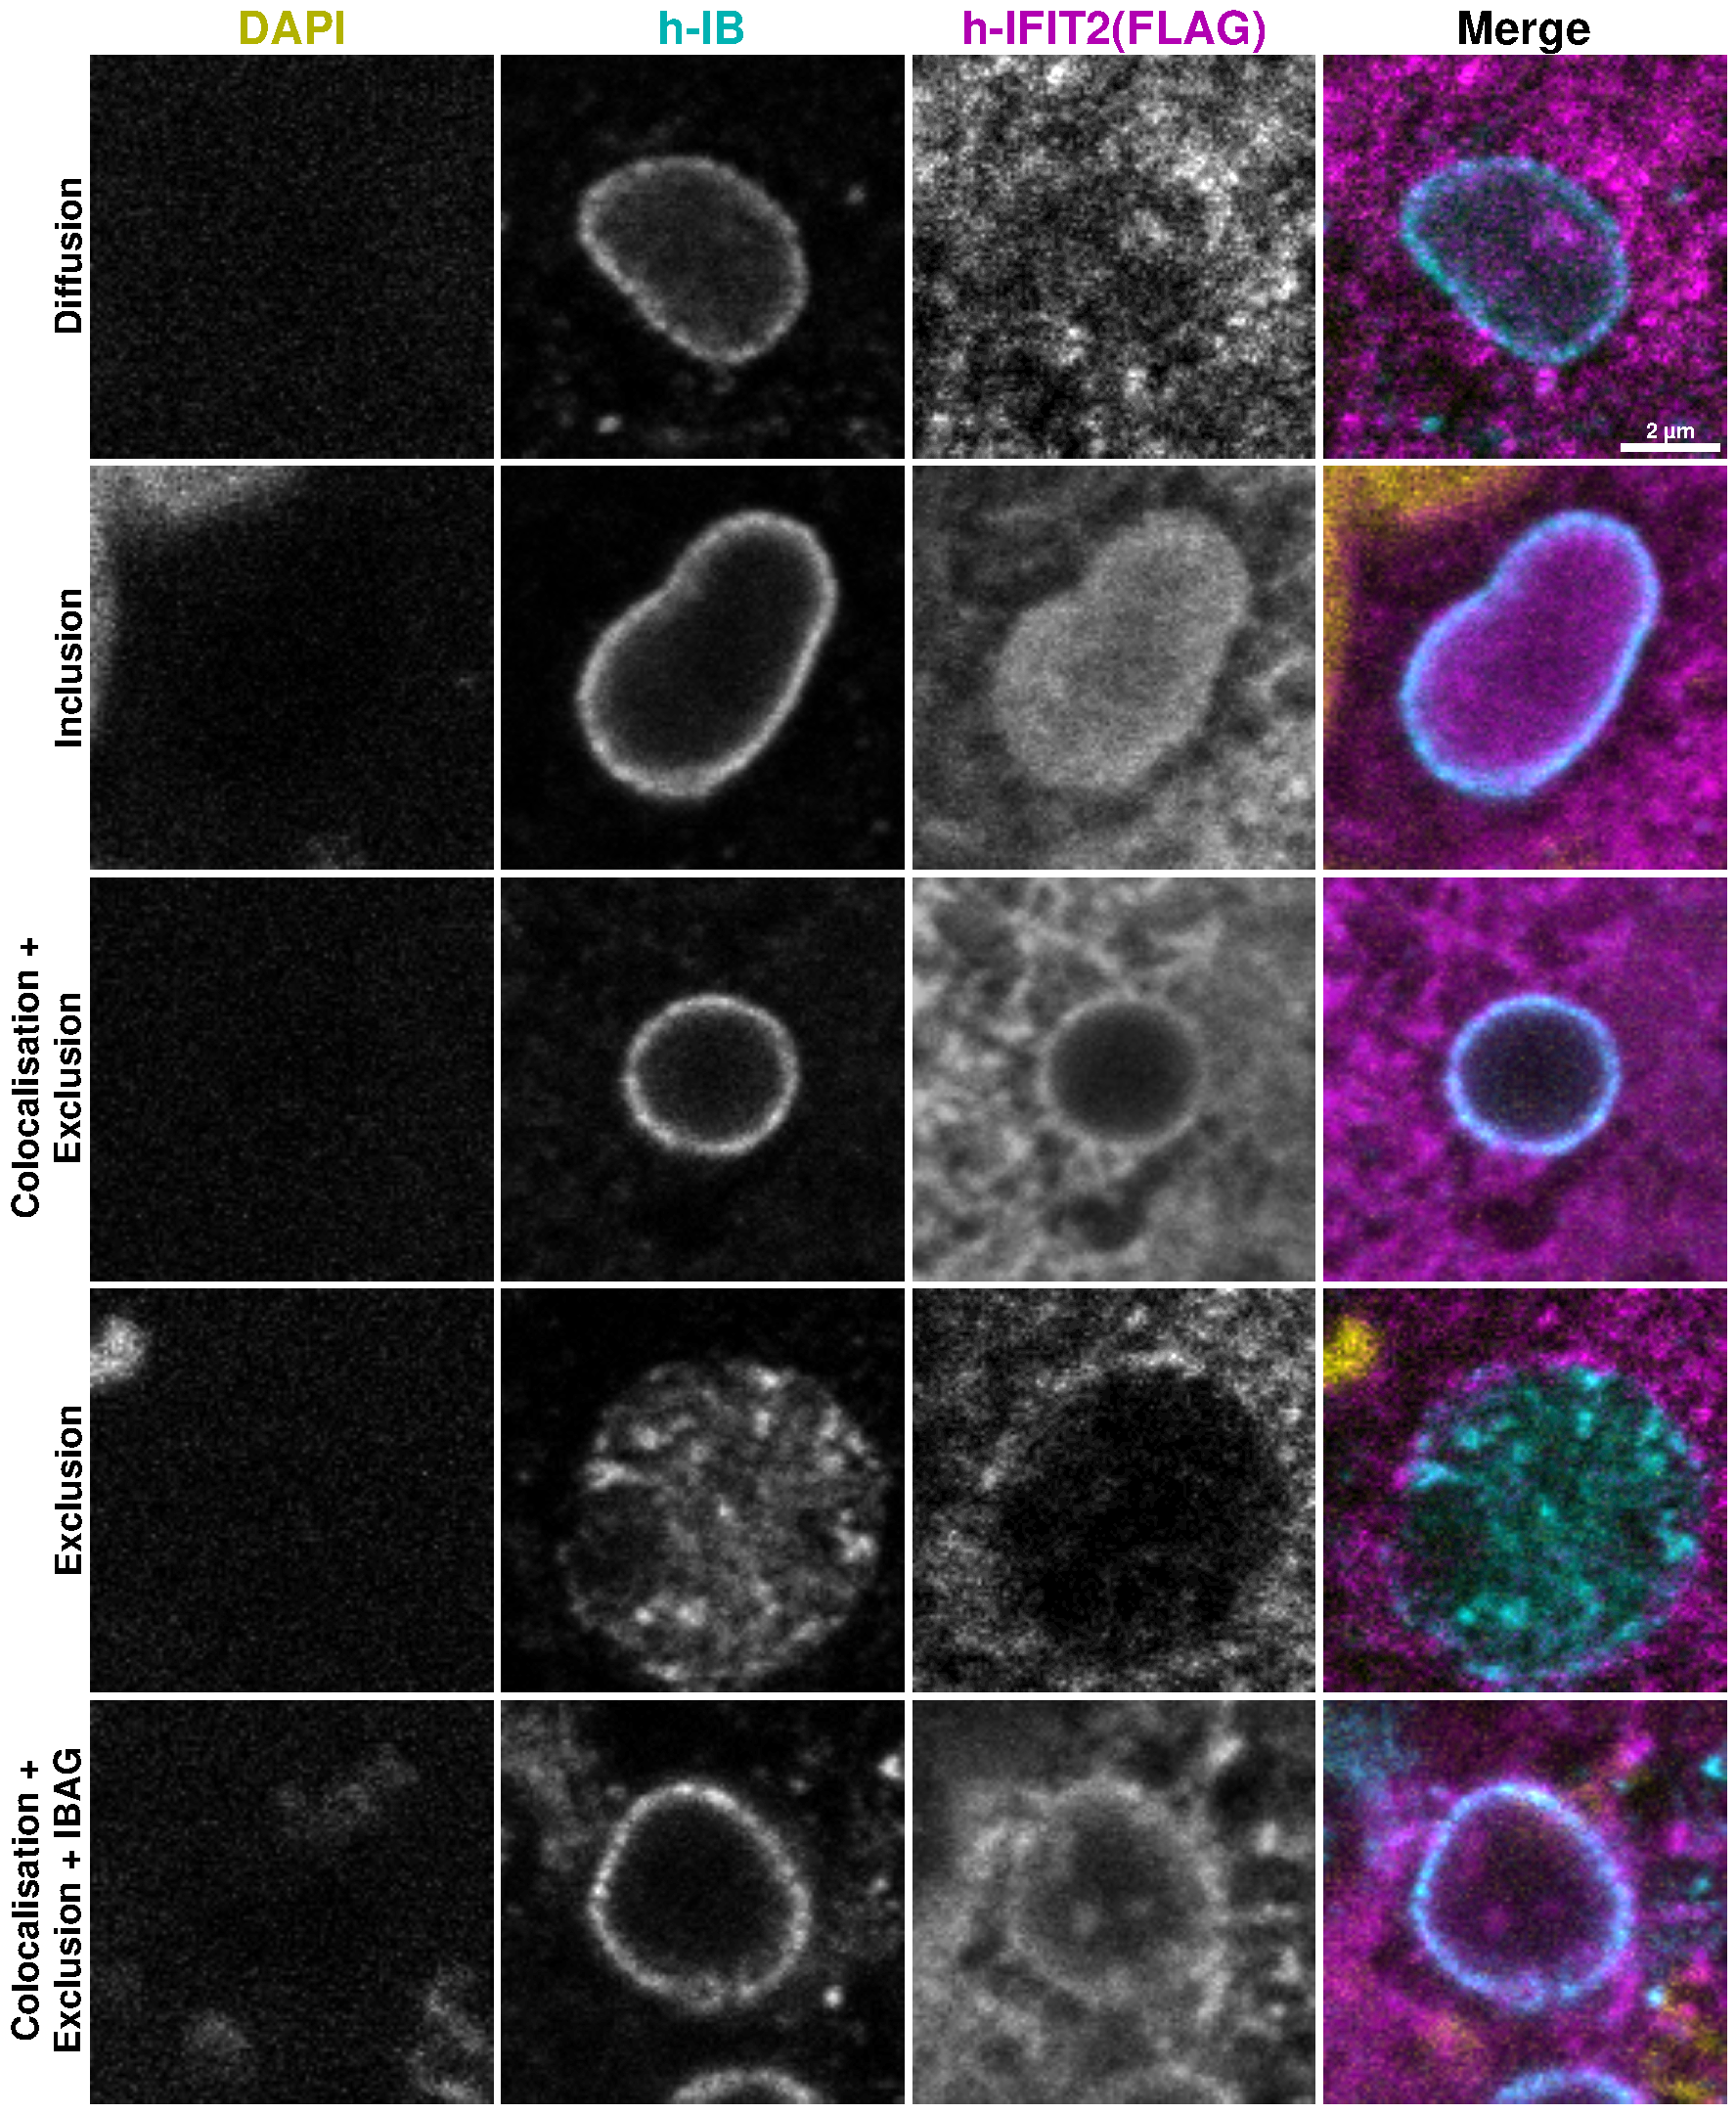
\includegraphics[width=1\linewidth]{09. Chapter 4/Figs/02. Overexpression/02. IFIT2/03. hi2f-hrsv.pdf}
    \caption[Representative Images of Observed Phenotypes of Exogenous hIFIT2 in the Context of hRSV Inclusion Bodies in Vero Cell Line.]{\textbf{Representative Images of Observed Phenotypes of Exogenous hIFIT2 in the Context of hRSV Inclusion Bodies in Vero Cell Line.} Vero cells were infected with human RSV at MOI 1. 24 HPI, the cells were transfected with hIFIT2-FLAG containing plasmids using TransIT-X2 and were fixed after a further 24 hours. Cellular nuclei were stained with DAPI (yellow), and cells were double-labelled with anti-RSV N (cyan) and anti-FLAG (magenta) antibodies. This figure showcases representative examples of relevant phenotypes in the interaction between exogenous hIFIT2 and hRSV inclusion bodies. These phenotypes are presented in descending order based on their percentage proportions. The scale bar indicates 2 \(\mu \mbox{m}\).}
    \label{fig:Representative Images of Observed Phenotypes of Exogenous hIFIT2 in the Context of hRSV Inclusion Bodies in Vero Cell Line}
\end{figure}

Subsequently, we endeavoured to validate the data acquired from exogenously expressed human and bovine IFIT2-FLAG in the context of human or bovine RSV pIBs by inducing the expression of human and bovine IFIT2-FLAG in hRSV- and bRSV-infected cells. The experimental methodology follows the description in Section \ref{subsec:Overexpressed IFIT1, IFIT3, and IFIT5 During RSV Infection}. In brief, Vero cells were initially infected with either human or bovine RSV at MOI 1 according to the standard protocol. At 24 HPI, the cells were transfected with either human or bovine IFIT2-FLAG-containing plasmids and were fixed after an additional 24 hours.

Initially, we examined the interaction phenotypes of exogenously expressed human IFIT2-FLAG with hRSV inclusion bodies, resulting in 155 observations. The frequencies of observed phenotypes, along with the IB sizes detected per phenotype occurring with a frequency higher than 5\%, are depicted in Figure \ref{fig:Observed Phenotypes of Exogenous hIFIT2 in the Context of hRSV Inclusion Bodies in Vero Cell Line}. Representative images of these phenotypes are shown in Figure \ref{fig:Representative Images of Observed Phenotypes of Exogenous hIFIT2 in the Context of hRSV Inclusion Bodies in Vero Cell Line}. A diverse range of interaction phenotypes was observed, with the most common being the diffusion phenotype occurring in 48\% of all observations. Following this, we observed inclusion (22\%), colocalisation associated with exclusion (14\%), exclusion (9\%), and colocalisation of IFIT2 with the IB boundary, while being excluded from the middle except for IFIT2 spots resembling IBAGs (5\% of all observations). Additionally, colocalisation and exclusion associated with the presence of IFIT2 spots within the IB boundary were observed in only 1\% of observations and thus were not included in the IB size analysis. Regarding the size of IBs associated with different phenotypes, a clear size separation based on median IB size is evident, although there is some overlap between phenotypes.

The diffusion phenotype predominantly occurred in smaller, sub-1 $\mu \mbox{m}^2$ IBs, with occurrences in medium-sized and large IBs (size range from 0.18 $\mu \mbox{m}^2$ to 19 $\mu \mbox{m}^2$, with a typical size of 0.9 $\mu \mbox{m}^2$). Inclusion-associated IBs ranged from 0.37 $\mu \mbox{m}^2$ to 19 $\mu \mbox{m}^2$, with a median value of 2.1 $\mu \mbox{m}^2$. Colocalisation associated with exclusion occurred in IBs ranging from 0.8 $\mu \mbox{m}^2$ to 25 $\mu \mbox{m}^2$, with a median value of 7 $\mu \mbox{m}^2$. The exclusion phenotype occurred in IBs ranging from 1.5 $\mu \mbox{m}^2$ to 130 $\mu \mbox{m}^2$, with a median size of 11 $\mu \mbox{m}^2$. These larger IBs often exhibited a distinct morphology compared to IBs associated with other phenotypes (Figure \ref{fig:Representative Images of Observed Phenotypes of Exogenous hIFIT2 in the Context of hRSV Inclusion Bodies in Vero Cell Line}), suggesting degradation of inclusion bodies. Lastly, colocalisation of IFIT2 with the IB boundary, while being excluded from the middle except for IFIT2 spots, occurred in very large IBs ranging from 11 $\mu \mbox{m}^2$ to 83 $\mu \mbox{m}^2$, with a median size of 32 $\mu \mbox{m}^2$.

In summary, these findings indicate that IFIT2 is associated with small (sub-1 $\mu \mbox{m}^2$) IBs predominantly through diffusion and occasionally forming inclusions. Medium-sized IBs (between 1 $\mu \mbox{m}^2$ and 10 $\mu \mbox{m}^2$) exhibit diffusion, inclusion, and colocalisation associated with exclusion phenotypes. Large IBs (above 10 $\mu \mbox{m}^2$) have the potential to display all phenotypic interactions, with predominant interaction phenotypes becoming colocalisation associated with exclusion (with or without spots) and the exclusion phenotype as their size increases. From the literature, we understand that as IBs increase in size, they mature, become more complex (e.g., the appearance of IBAGs), and their structure becomes more gel-like \cite{Weber1995NonstructuralSerum, Fricke2013P38Assembly, Rincheval2017FunctionalVirus, Jobe2021BovineResponses}. This suggests that the interaction of exogenous human IFIT2 with hRSV inclusion bodies depends on their maturation level. Furthermore, this data indicates that IFIT2 exhibits an approximately equal frequency of phenotypes suggesting IB interaction (inclusion and colocalisation) and those implying no or minimal interaction (diffusion and exclusion). Overall, this data replicates what was observed with endogenous human and bovine IFIT2s during RSV infection or human and monkey IFIT2 in the context of RSV pIBs, assuming that IFIT2(A) and IFIT2(B) antibodies collectively detect the entire IFIT2 population.

\begin{figure}
    \begin{subfigure}{0.495\textwidth}
        \caption{}
        \includegraphics[width=1\linewidth]{09. Chapter 4/Figs/02. Overexpression/02. IFIT2/04. bar_bi2f_hrsv.pdf} 
    \end{subfigure}
    \begin{subfigure}{0.495\textwidth}
        \caption{}
        \includegraphics[width=1\linewidth]{09. Chapter 4/Figs/02. Overexpression/02. IFIT2/05. box_bi2f_hrsv.pdf}
    \end{subfigure}
    \caption[Observed Phenotypes of Exogenous bIFIT2 in the Context of hRSV Inclusion Bodies in Vero Cell Line.]{\textbf{Observed Phenotypes of Exogenous bIFIT2 in the Context of hRSV Inclusion Bodies in Vero Cell Line.} Vero cells were infected with human RSV at MOI 1. 24 HPI, the cells were transfected with bIFIT2-FLAG containing plasmids using TransIT-X2 and were fixed after a further 24 hours. Cells were labelled with anti-RSV N and anti-FLAG antibodies and imaged on a confocal microscope. Panel (a) shows the percentual proportions of observed phenotypes between hRSV inclusion bodies and exogenous bIFIT2 (62 observations), with the red dotted line denoting the 5\% threshold, marking phenotypes considered relevant above this limit. Panel (b) shows the IB area in \(\mu \mbox{m}^2\) per observed relevant phenotype.}
    \label{fig:Observed Phenotypes of Exogenous bIFIT2 in the Context of hRSV Inclusion Bodies in Vero Cell Line}
\end{figure}

\begin{figure}
    \centering
    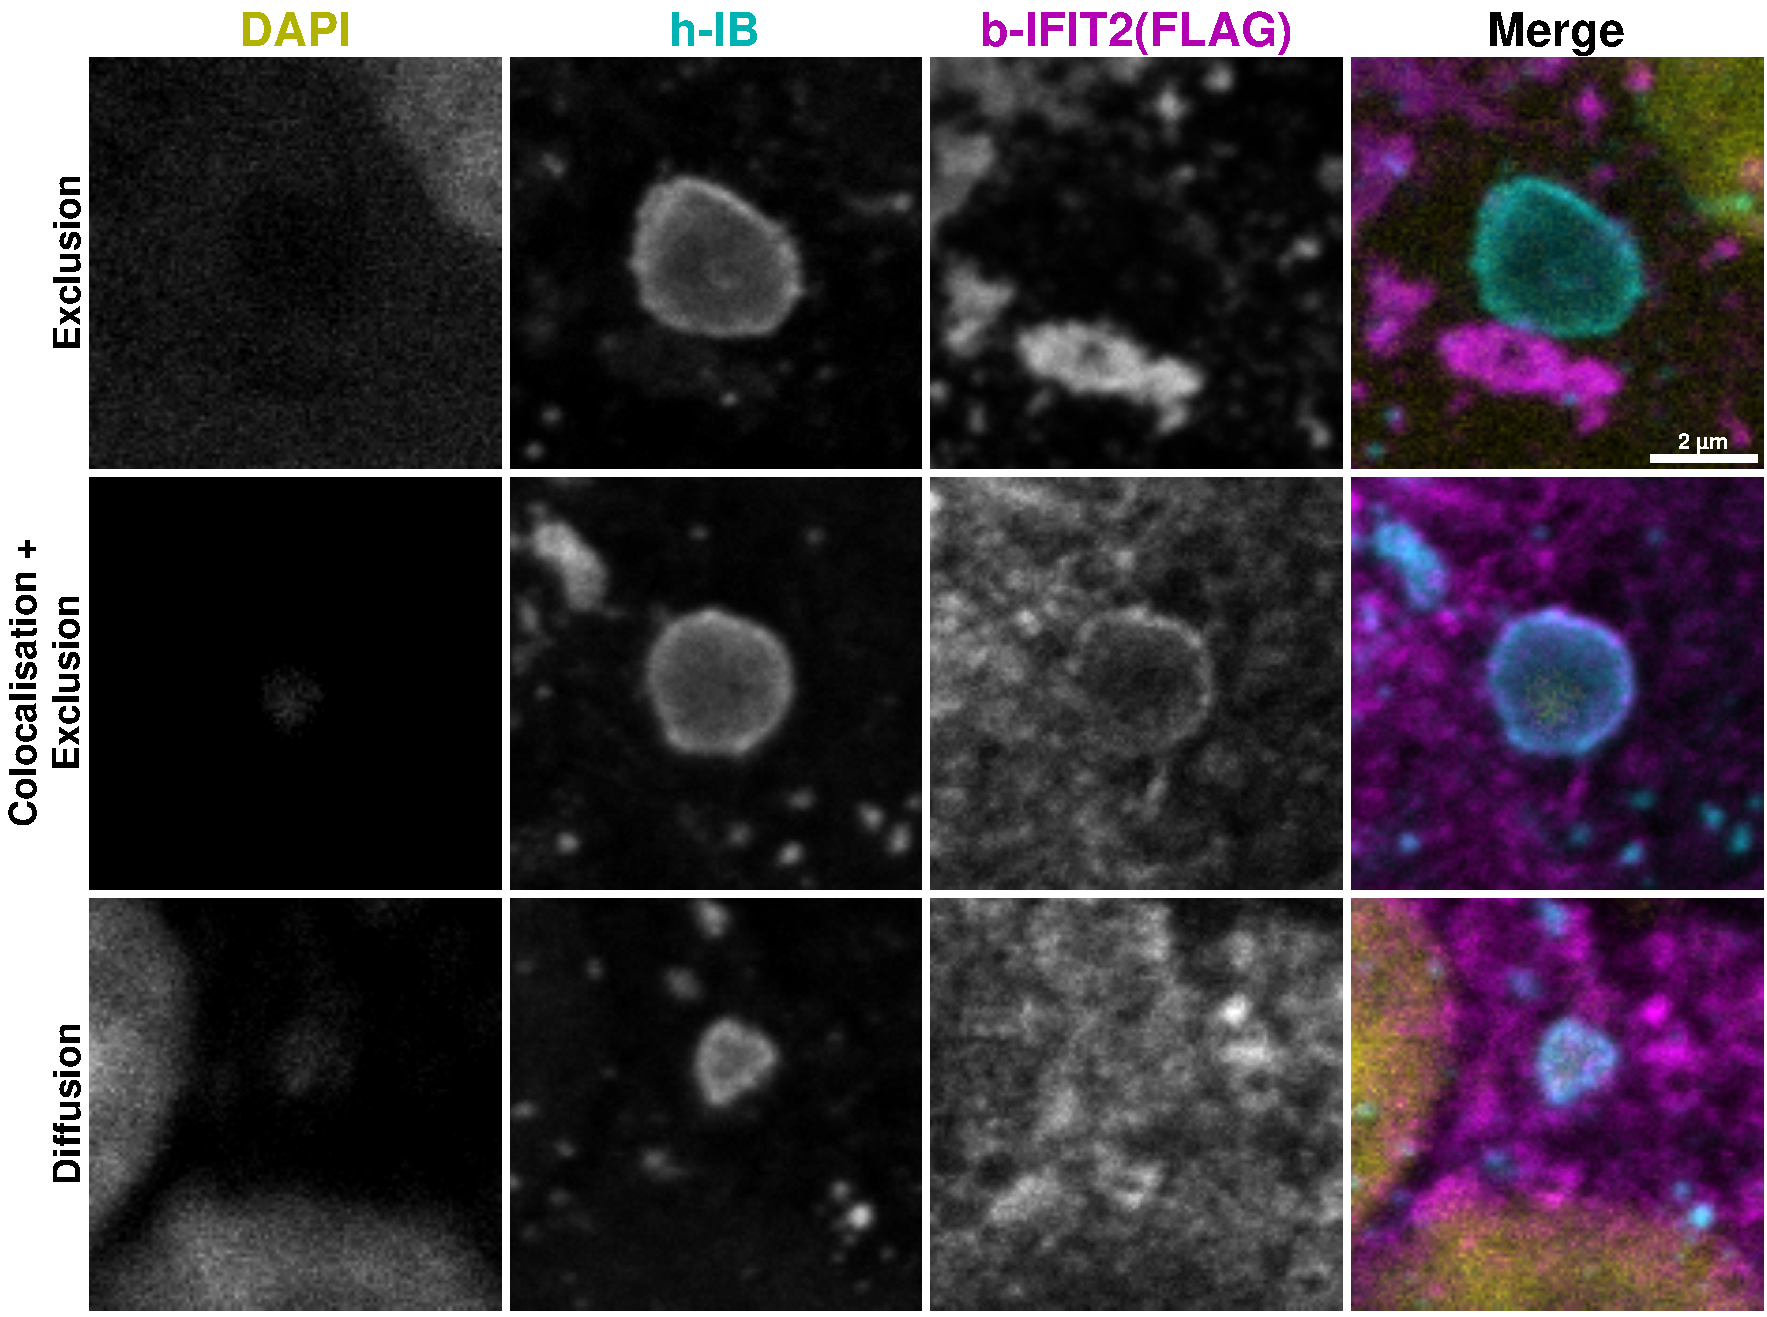
\includegraphics[width=1\linewidth]{09. Chapter 4/Figs/02. Overexpression/02. IFIT2/06. bi2f-hrsv.pdf}
    \caption[Representative Images of Observed Phenotypes of Exogenous bIFIT2 in the Context of hRSV Inclusion Bodies in Vero Cell Line.]{\textbf{Representative Images of Observed Phenotypes of Exogenous bIFIT2 in the Context of hRSV Inclusion Bodies in Vero Cell Line.} Vero cells were infected with human RSV at MOI 1. 24 HPI, the cells were transfected with bIFIT2-FLAG containing plasmids using TransIT-X2 and were fixed after a further 24 hours. Cellular nuclei were stained with DAPI (yellow), and cells were double-labelled with anti-RSV N (cyan) and anti-FLAG (magenta) antibodies. This figure showcases representative examples of relevant phenotypes in the interaction between exogenous bIFIT2 and hRSV inclusion bodies. These phenotypes are presented in descending order based on their percentage proportions. The scale bar indicates 2 \(\mu \mbox{m}\).}
    \label{fig:Representative Images of Observed Phenotypes of Exogenous bIFIT2 in the Context of hRSV Inclusion Bodies in Vero Cell Line}
\end{figure}

Next, we set to investigate the interaction of exogenously expressed human IFIT2-FLAG with bRSV inclusion bodies. Despite numerous attempts, we were unable to observe a single co-infected/transfected cell. Consequently, we redirected our attention to the examination of exogenously expressed bovine IFIT2-FLAG and its localisation with hRSV inclusion bodies. Within the 62 detected bIFIT2/hRSV IB interactions, we identified three distinct interaction phenotypes. The frequencies of occurrences for each phenotype, along with the IB sizes per phenotype, are illustrated in Figure \ref{fig:Observed Phenotypes of Exogenous bIFIT2 in the Context of hRSV Inclusion Bodies in Vero Cell Line}. Representative images of these bIFIT2/hRSV IB interactions are displayed in Figure \ref{fig:Representative Images of Observed Phenotypes of Exogenous bIFIT2 in the Context of hRSV Inclusion Bodies in Vero Cell Line}. The most frequently occurring interaction phenotype was exclusion, observed in 66\% of observations. The sizes of IBs associated with this phenotype spanned the entire IB size spectrum, ranging from 0.11 $\mu \mbox{m}^2$ to 30 $\mu \mbox{m}^2$, with a typical size of 1 $\mu \mbox{m}^2$. The next most frequent phenotype was colocalisation associated with exclusion, observed in 17\% of all observations. This phenotype predominantly occurred in larger IBs, ranging in size from 0.7 $\mu \mbox{m}^2$ to 15 $\mu \mbox{m}^2$, with a median size of 5 $\mu \mbox{m}^2$. Lastly, bIFIT2 was observed to be diffused equally between the cytoplasm and IB structures in 16\% of the observations. The diffusion-associated IBs were of smaller size, ranging from 0.12 $\mu \mbox{m}^2$ to 1.3 $\mu \mbox{m}^2$, with a median value of 0.55 $\mu \mbox{m}^2$. Overall, the exclusion phenotype was the most common and occurred across the entire size spectrum. The remaining third of bIFIT2/hRSV IB interactions was almost equally divided between colocalisation associated with exclusion and the diffusion phenotype, occurring in a size-specific manner.

\begin{figure}
    \begin{subfigure}{0.495\textwidth}
        \caption{}
        \includegraphics[width=1\linewidth]{09. Chapter 4/Figs/02. Overexpression/02. IFIT2/07. bar_bi2f_brsv.pdf} 
    \end{subfigure}
    \begin{subfigure}{0.495\textwidth}
        \caption{}
        \includegraphics[width=1\linewidth]{09. Chapter 4/Figs/02. Overexpression/02. IFIT2/08. box_bi2f_brsv.pdf}
    \end{subfigure}
    \caption[Observed Phenotypes of Exogenous bIFIT2 in the Context of bRSV Inclusion Bodies in Vero Cell Line.]{\textbf{Observed Phenotypes of Exogenous bIFIT2 in the Context of bRSV Inclusion Bodies in Vero Cell Line.} Vero cells were infected with human RSV at MOI 1. 24 HPI, the cells were transfected with bIFIT2-FLAG containing plasmids using TransIT-X2 and were fixed after a further 24 hours. Cells were labelled with anti-RSV N and anti-FLAG antibodies and imaged on a confocal microscope. Panel (a) shows the percentual proportions of observed phenotypes between bRSV inclusion bodies and exogenous bIFIT2 (31 observations), with the red dotted line denoting the 5\% threshold, marking phenotypes considered relevant above this limit. Panel (b) shows the IB area in \(\mu \mbox{m}^2\) per observed relevant phenotype.}
    \label{fig:Observed Phenotypes of Exogenous bIFIT2 in the Context of bRSV Inclusion Bodies in Vero Cell Line}
\end{figure}

\begin{figure}
    \centering
    \includegraphics[width=1\linewidth]{09. Chapter 4/Figs/02. Overexpression/02. IFIT2/09. bi2f-brsv.pdf}
    \caption[Representative Images of Observed Phenotypes of Exogenous bIFIT2 in the Context of bRSV Inclusion Bodies in Vero Cell Line.]{\textbf{Representative Images of Observed Phenotypes of Exogenous bIFIT2 in the Context of bRSV Inclusion Bodies in Vero Cell Line.} Vero cells were infected with human RSV at MOI 1. 24 HPI, the cells were transfected with bIFIT2-FLAG containing plasmids using TransIT-X2 and were fixed after a further 24 hours. Cellular nuclei were stained with DAPI (yellow), and cells were double-labelled with anti-RSV N (cyan) and anti-FLAG (magenta) antibodies. This figure showcases representative examples of relevant phenotypes in the interaction between exogenous bIFIT2 and bRSV inclusion bodies. These phenotypes are presented in descending order based on their percentage proportions. The scale bar indicates 2 \(\mu \mbox{m}\).}
    \label{fig:Representative Images of Observed Phenotypes of Exogenous bIFIT2 in the Context of bRSV Inclusion Bodies in Vero Cell Line}
\end{figure}

Finally, we have investigated the interaction of exogenously expressed bovine IFIT2-FLAG with bRSV inclusion bodies. We have obtained 31 IB/bIFIT2 interaction observations. The frequencies of the interaction observed intraction phenotypes, along with the IB sizes assocated with these phenotypes is shown in Figure \ref{fig:Observed Phenotypes of Exogenous bIFIT2 in the Context of bRSV Inclusion Bodies in Vero Cell Line}. The representative images of these phenotypes are shown in Figure \ref{fig:Representative Images of Observed Phenotypes of Exogenous bIFIT2 in the Context of bRSV Inclusion Bodies in Vero Cell Line}. In the majority of cases (94\%) we have observed exogenous bIFIT2 to be excluded from bRSV IBs. These occured in both small and large IBs, which ranged from 0.54 \(\mu \mbox{m}^2\) to 37 \(\mu \mbox{m}^2\), with a atypical size of 3.9 \(\mu \mbox{m}^2\). We also obtained two obsevations of diffusion phenotype which were 0.8 \(\mu \mbox{m}^2\) and 1.8 \(\mu \mbox{m}^2\) in size. ...

94 6

0.54 3.9 37
0.8 1.8

maybe if more large ones we would see coloc + excl

summary

paragraph of putting infection and all 2 together

prepare for rbm - positive interaction could be mediated via i2-rna interaction

\subsection{Endeavour in Understanding the Mechanisms of IFIT2-RSV IB Interaction} \label{subsec:Endeavour in Understanding the Mechanisms of IFIT2-RSV IB Interaction}
%The Generation of Bovine IFIT2 RNA-Binding Mutant
Using published data about hIFIT2 rna-binding mutant

Difficulty of using alpha-fold with IFIT2 due to the swap domain

Using SWISS-MODEL to predict bIFIT2 structure from published hIFIT2 structures

Alignment of both structures, assessment of electrostatic charges and establishment of residues to be mutated

Primer design and mutagenesis procedure based on published hIFIT2 RNA-binding mutant paper
\cite{Tran2020InfluenzaMRNAs}

\ref{subsec:PCR for Point Mutant Generation}

\begin{figure}
    \centering
    \includegraphics[width=1\linewidth]{09. Chapter 4/Figs/01. pIB/03. IFIT2/05. IFIT2-RNA binding mutant/01. Structure/01. structure.png}
    \caption[ifit2 mutant structure]{\textbf{bifit2 mutant structure.} write caption}
    \label{fig:ifit2 mutant structure}
\end{figure}






\begin{figure}
    \begin{subfigure}{0.495\textwidth}
        \caption{}
        \includegraphics[width=1\linewidth]{09. Chapter 4/Figs/01. pIB/03. IFIT2/05. IFIT2-RNA binding mutant/02. pIB/01. bar_bi2f24_hnhp.pdf} 
    \end{subfigure}
    \begin{subfigure}{0.495\textwidth}
        \caption{}
        \includegraphics[width=1\linewidth]{09. Chapter 4/Figs/01. pIB/03. IFIT2/05. IFIT2-RNA binding mutant/02. pIB/02. box_bi2f24_hnhp.pdf}
    \end{subfigure}
    \caption[Diverse Phenotypic Interactions of Bovine IFIT2 RNA-Binding Mutant with Human RSV Pseudo Inclusion Bodies (pIBs) in the Vero Cell Line.]{\textbf{Diverse Phenotypic Interactions of Bovine IFIT2 RNA-Binding Mutant with Human RSV Pseudo Inclusion Bodies (pIBs) in the Vero Cell Line.} Vero cells were transfected with hRSV N and P, along with bovine IFIT2-FLAG RNA-binding mutant containing plasmids using TransIT-X2 and were fixed after 24 hours. Cells were labelled with anti-RSV N and anti-FLAG antibodies and imaged on a confocal microscope. Panel (a) shows percentual proportions of observed phenotypes between hRSV pseudo inclusion bodies and exogenous bovine IFIT2-FLAG RNA-binding mutant (548 observations), with the red dotted line denoting the 5\% threshold, marking phenotypes considered relevant above this limit. Panel (b) shows the IB area in \(\mu \mbox{m}^2\) per observed relevant phenotype.}
    \label{fig:Diverse Phenotypic Interactions of Bovine IFIT2 RNA-Binding Mutant with Human RSV Pseudo Inclusion Bodies (pIBs) in the Vero Cell Line}
\end{figure}

\begin{figure}
    \centering
    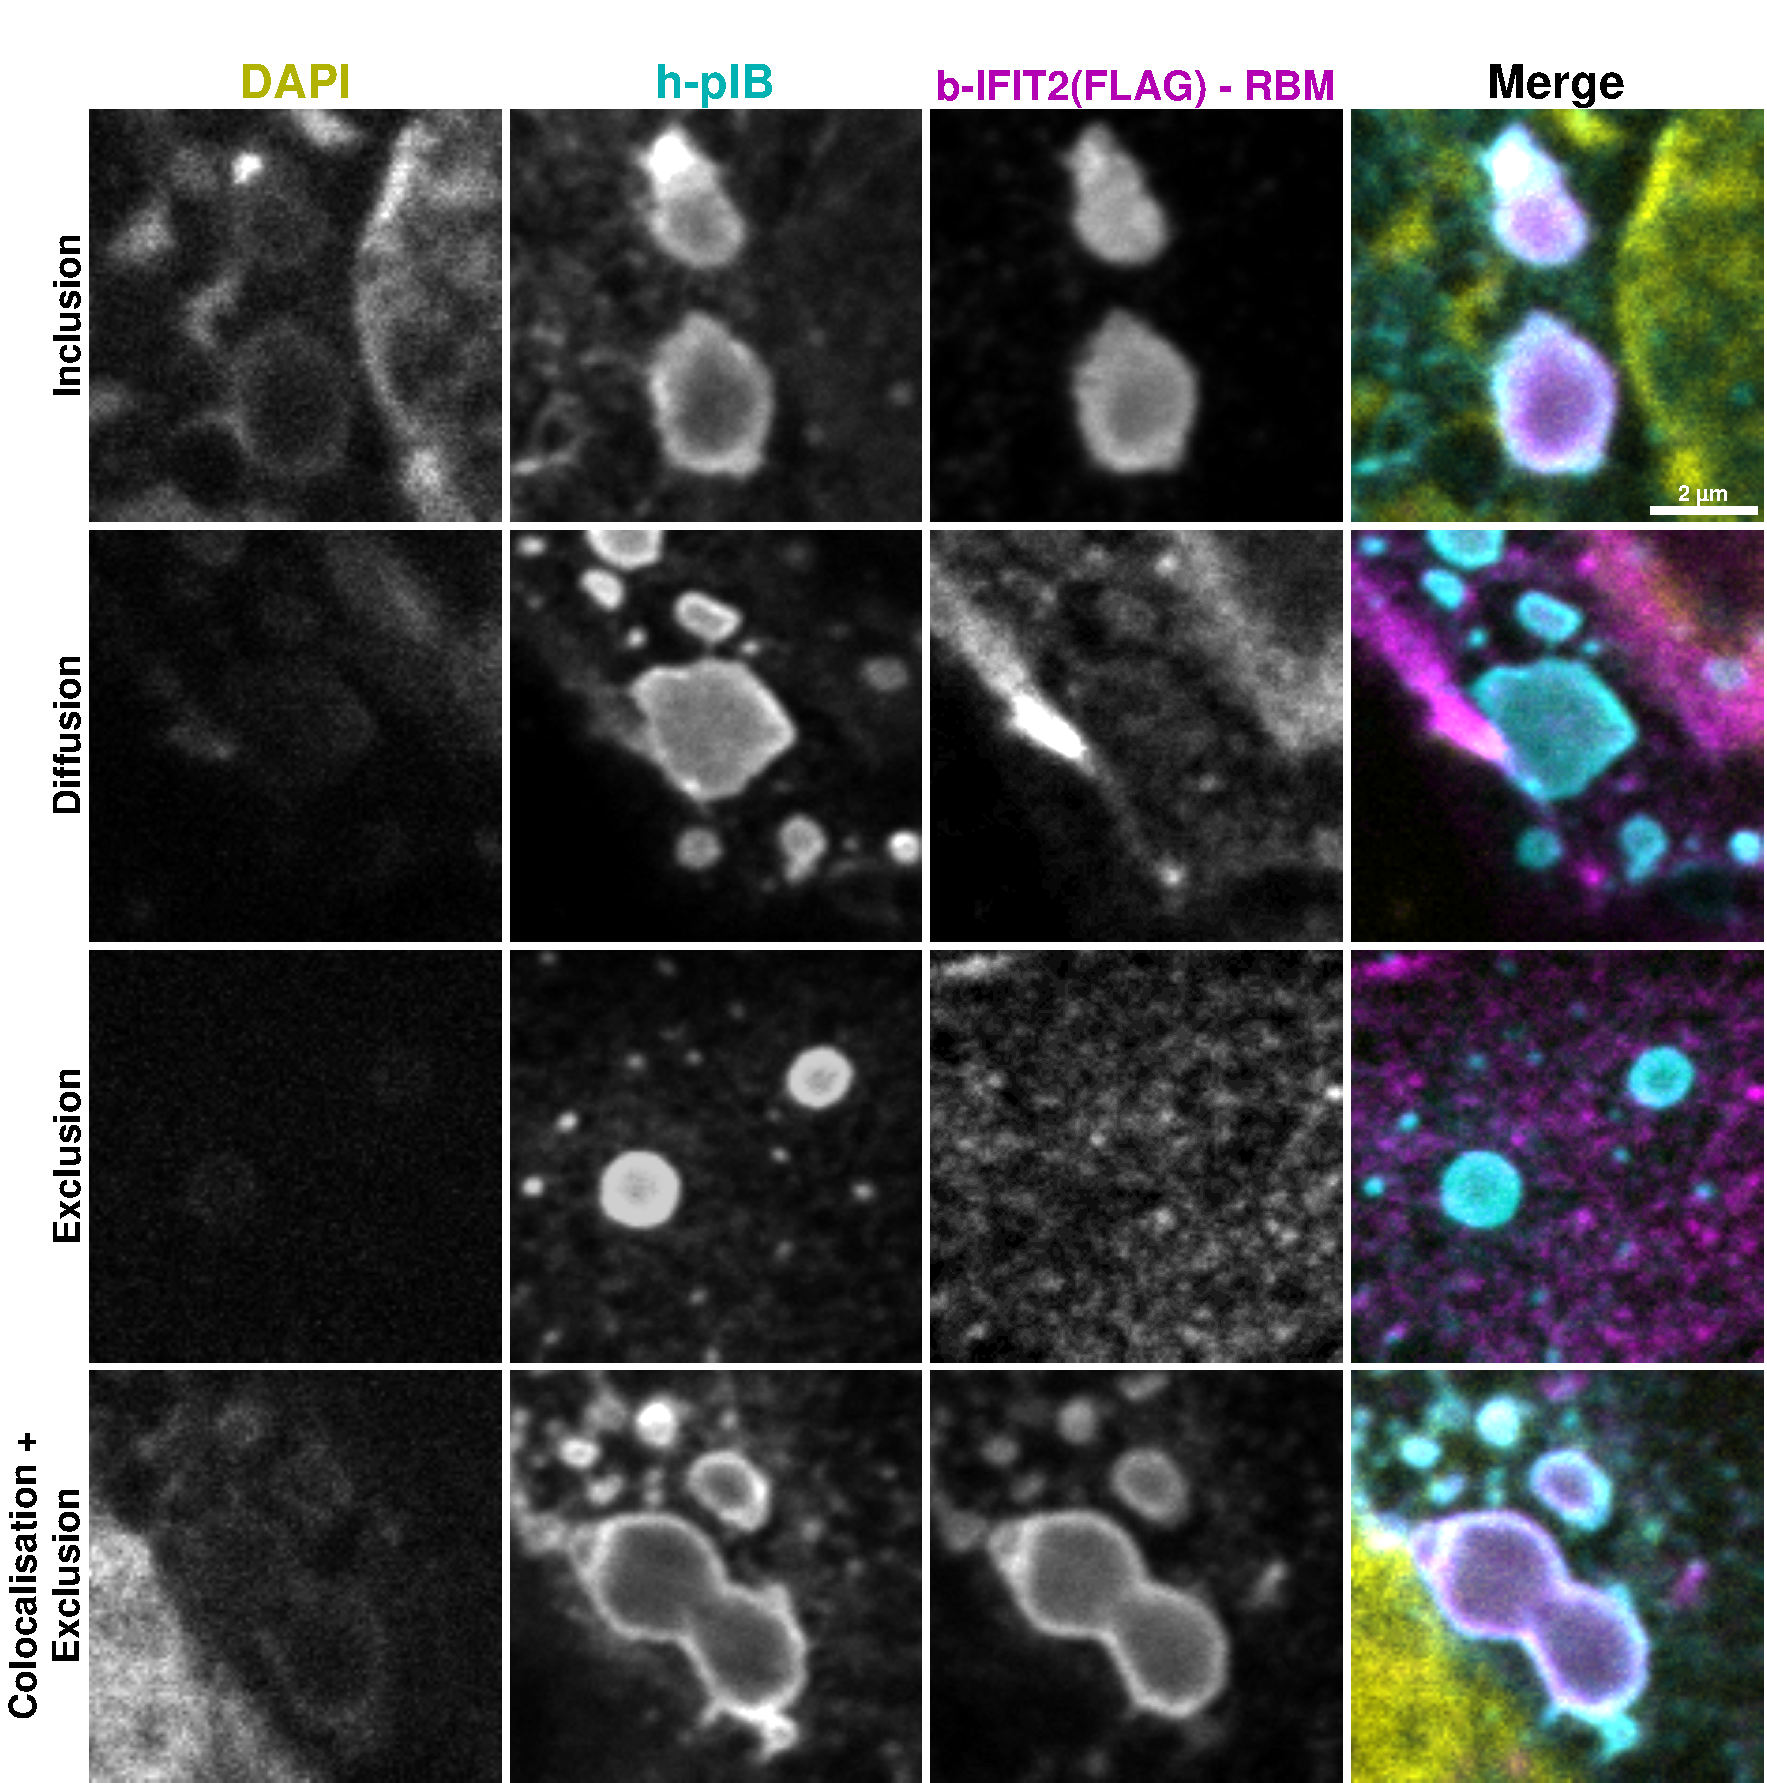
\includegraphics[width=1\linewidth]{09. Chapter 4/Figs/01. pIB/03. IFIT2/05. IFIT2-RNA binding mutant/02. pIB/03. bi2f24-hnhp.pdf}
    \caption[Representative Images of Diverse Phenotypic Interactions of Bovine IFIT2 RNA-Binding Mutant with Human RSV Pseudo Inclusion Bodies (pIBs) in the Vero Cell Line.]{\textbf{Representative Images of Diverse Phenotypic Interactions of Bovine IFIT2 RNA-Binding Mutant with Human RSV Pseudo Inclusion Bodies (pIBs) in the Vero Cell Line.}  Vero cells were transfected with bRSV N and P, along with bovine IFIT2-FLAG RNA-binding mutant containing plasmids using TransIT-X2 and were fixed after 24 hours. Cellular nuclei were stained with DAPI (yellow), and cells were double-labelled with anti-RSV N (cyan) and anti-FLAG (magenta) antibodies. This figure showcases representative examples of relevant phenotypes in the interaction between exogenous bovine IFIT2-FLAG RNA-binding mutant and hRSV pseudo-inclusion bodies. These phenotypes are presented in descending order based on their percentage proportions. The scale bar indicates 2 \(\mu \mbox{m}\).}
    \label{fig:Representative Images of Diverse Phenotypic Interactions of Bovine IFIT2 RNA-Binding Mutant with Human RSV Pseudo Inclusion Bodies (pIBs) in the Vero Cell Line}
\end{figure}

49 27 13 11

0.12 0.8 19
0.12 0.5 8.5
0.19 1 140
0.31 1.8 40

\begin{figure}
    \begin{subfigure}{0.495\textwidth}
        \caption{}
        \includegraphics[width=1\linewidth]{09. Chapter 4/Figs/01. pIB/03. IFIT2/05. IFIT2-RNA binding mutant/02. pIB/04. bar_bi2f24_bnbp.pdf} 
    \end{subfigure}
    \begin{subfigure}{0.495\textwidth}
        \caption{}
        \includegraphics[width=1\linewidth]{09. Chapter 4/Figs/01. pIB/03. IFIT2/05. IFIT2-RNA binding mutant/02. pIB/05. box_bi2f24_bnbp.pdf}
    \end{subfigure}
    \caption[Diverse Phenotypic Interactions of Bovine IFIT2 RNA-Binding Mutant with Bovine RSV Pseudo Inclusion Bodies (pIBs) in the Vero Cell Line.]{\textbf{Diverse Phenotypic Interactions of Bovine IFIT2 RNA-Binding Mutant with Bovine RSV Pseudo Inclusion Bodies (pIBs) in the Vero Cell Line.} Vero cells were transfected with bRSV N and P, along with bovine IFIT2-FLAG RNA-binding mutant containing plasmids using TransIT-X2 and were fixed after 24 hours. Cells were labelled with anti-RSV N and anti-FLAG antibodies and imaged on a confocal microscope. Panel (a) shows percentual proportions of observed phenotypes between bRSV pseudo inclusion bodies and exogenous bovine IFIT2-FLAG RNA-binding mutant (2 observations), with the red dotted line denoting the 5\% threshold, marking phenotypes considered relevant above this limit. Panel (b) shows the IB area in \(\mu \mbox{m}^2\) per observed relevant phenotype.}
    \label{fig:Diverse Phenotypic Interactions of Bovine IFIT2 RNA-Binding Mutant with Bovine RSV Pseudo Inclusion Bodies (pIBs) in the Vero Cell Line}
\end{figure}

\begin{figure}
    \centering
    \includegraphics[width=1\linewidth]{09. Chapter 4/Figs/01. pIB/03. IFIT2/05. IFIT2-RNA binding mutant/02. pIB/06. bi2f24-bnbp.pdf}
    \caption[Representative Images of Diverse Phenotypic Interactions of Bovine IFIT2 RNA-Binding Mutant with Bovine RSV Pseudo Inclusion Bodies (pIBs) in the Vero Cell Line.]{\textbf{Representative Images of Diverse Phenotypic Interactions of Bovine IFIT2 RNA-Binding Mutant with Bovine RSV Pseudo Inclusion Bodies (pIBs) in the Vero Cell Line.}  Vero cells were transfected with bRSV N and P, along with bovine IFIT2-FLAG RNA-binding mutant containing plasmids using TransIT-X2 and were fixed after 24 hours. Cellular nuclei were stained with DAPI (yellow), and cells were double-labelled with anti-RSV N (cyan) and anti-FLAG (magenta) antibodies. This figure showcases representative examples of relevant phenotypes in the interaction between exogenous bovine IFIT2-FLAG RNA-binding mutant and bRSV pseudo inclusion bodies. These phenotypes are presented in descending order based on their percentage proportions. The scale bar indicates 2 \(\mu \mbox{m}\).}
    \label{fig:Representative Images of Diverse Phenotypic Interactions of Bovine IFIT2 RNA-Binding Mutant with Bovine RSV Pseudo Inclusion Bodies (pIBs) in the Vero Cell Line}
\end{figure}

100

0.6 2.9


transfecting bi2f24 + bngfp + p inhibits bpIBs (compared to hi2f or bi2f)

% summary i2
We have described how bovine IFIT2 RNA-binding mutant was designed based on the published human IFIT2 RNA-binding mutant data (needs to be annotated more). Overexpression of bovine IFIT2 RNA-binding mutant yields cellular distribution and morphology similar to what was observed with overexpressing human IFIT2-FLAG, suggesting that the mutant proteins are not toxic to the cells. In the first experiment where we were looking at interaction between bovine IFIT2 RNA-binding mutant and human pseudo inclusion bodies we saw several phenotypes. We observed bovine IFIT2 RNA-binding mutant being excluded from small and big pIBs and pIB associated filamentous network, while fully or partially colocalising with other pIBs. In a subsequent experiment we observed only colocalization and inclusion formation. When assessing the interaction between bovine IFIT2 RNA-binding mutant and human pIBs formed using wild-type human RSV P and GFP-tagged human RSV N, we observed consistently in two experiments that bovine IFIT2 RNA-binding mutant colocalises to the pIB structures.